\documentclass[12pt,preprint]{aastex}
%\documentclass[preprint]{aastex}

\bibliographystyle{apj}
\newcommand{\etal}{et al.}



\usepackage[textwidth=0.8in,colorinlistoftodos]{todonotes}

% for highlighting text
\usepackage{framed}
\colorlet{shadecolor}{yellow} 

%#For adding line numbers:
\usepackage{lineno}
\linenumbers


%\usepackage{rotating}
\usepackage{amsmath}
\usepackage{graphicx}
\usepackage{xspace}
\usepackage{url}

% Note, hyperref has to come after other packages!
\usepackage{hyperref}

% some units
\newcommand{\kev}{\text{Kev}\xspace}
\newcommand{\mev}{\text{MeV}\xspace}
\newcommand{\gev}{\text{GeV}\xspace}
\newcommand{\tev}{\text{TeV}\xspace}
\newcommand{\sr}{\text{sr}\xspace}
\newcommand{\s}{\text{s}\xspace}
\newcommand{\ph}{\text{ph}\xspace}
\newcommand{\cm}{\text{cm}\xspace}
\renewcommand{\sec}{\text{s}\xspace}
\newcommand{\tsext}{{\ensuremath{\text{TS}_{\text{ext}}}}\xspace}
\newcommand{\tsinc}{\ensuremath{\text{TS}_{\text{inc}}}\xspace}
\newcommand{\loglikelihood}{\ensuremath{LL}\xspace}
\newcommand{\chandra}{\text{{\em Chandra}}\xspace}
\newcommand{\swiftxrt}{\text{{\em Swift}/XRT}\xspace}
\newcommand{\rosat}{\text{{\em ROSAT}}\xspace}
\newcommand{\suzaku}{\text{{\em Suzaku}}\xspace}
\newcommand{\asca}{\text{{\em ASCA}}\xspace}
\newcommand{\einstein}{\text{{\em Einstein}}\xspace}
\newcommand{\xmmnewton}{\text{{\em XMM-Newton}}\xspace}

\newcommand{\rsixeight}{{\ensuremath{\text{r}_{68}}}\xspace}

\newcommand{\tsextpointlike}{\ensuremath{\tsext_{,\pointlike}}\xspace}
\newcommand{\tsextgtlike}{\ensuremath{\tsext_{,\gtlike}}\xspace}

\newcommand{\ts}{\text{TS}\xspace}
\newcommand{\glon}{\text{GLON}\xspace}
\newcommand{\glat}{\text{GLAT}\xspace}
\newcommand{\altdiff}{\text{alt,diff}\xspace}
\newcommand{\altpsf}{\text{alt,psf}\xspace}
\newcommand{\sys}{\text{sys}\xspace}
\newcommand{\stat}{\text{stat}\xspace}

\renewcommand{\deg}{\ensuremath{^\circ}\xspace}

% the program names
\newcommand{\pointlike}{\text{\em pointlike}\xspace}
\newcommand{\python}{\text{\em python}\xspace}
\newcommand{\gtlike}{\text{\em gtlike}\xspace}
\newcommand{\gtobssim}{\text{\em gtobssim}\xspace}
\newcommand{\minuit}{\text{\em Minuit}\xspace}
\renewcommand{\approx}{\sim\!\xspace}

\shorttitle{Search for Extended LAT Sources}

\begin{document}

\title{Search for Spatially Extended Fermi-LAT Sources Using Two Years of Flight
Data}

\author{
J.~Lande\altaffilmark{3}, 
\altaffiltext{3}{W. W. Hansen Experimental Physics Laboratory, Kavli Institute for Particle Astrophysics and Cosmology, Department of Physics and SLAC National Accelerator Laboratory, Stanford University, Stanford, CA 94305, USA}
}


\begin{abstract}
We present a new method for analyzing 
the spatial extension of sources with
the Large Area Telescope (LAT), the primary science instrument on the
{\em Fermi Gamma-ray Space Telescope (Fermi)}. 
The source extension is an important input to correctly 
associate LAT sources with their counterparts at other
wavelengths. We provide
a series of Monte Carlo studies to validate this tool and calculate
the LAT's detection threshold to spatially extended sources.  We then
apply this tool to test all sources in the two year source catalog for
extension. We present on the detection of nine spatially extended sources
in addition to the twelve spatially extended sources reported in the
second Fermi-LAT Catalog (2FGL).
\end{abstract}

\listoftodos

\section{Introduction}

The Large Area Telescope (LAT) is a pair conversion telescope on the Fermi
Gamma-Ray Space Telescope (FGST). It has been surveying the $\gamma$-ray
sky since June 2008.  Fermi has a broad energy coverage (20 \mev to $>300$
\gev), wide field of view ($\approx 2.4 \sr$), and large effective area
($\approx 8000 \cm^2$ at $>1 \gev$).

Using two years of all sky surveying data, the LAT Collaboration published
a catalog of 1873 \gev sources \citep{second_cat}. Many of these can be
positionally associated with a variety of source classes including Active
Galactic Nuclei (AGN), pulsars, galaxies, and supernova remnants (SNRs).
While many of the LAT sources can be spatially resolved when observed
at other frequencies, detection of an extension at \gev energies by
the LAT is complicated by the rather large point-spread function (PSF)
of the instrument. The angular resolution for events converting in the
front part of the detector, defined as the 68\% containment radius for
a point source, is approximately $3.5^{\circ}$ at 100 \mev, improving
to about 0.1$^{\circ}$ at 10 \gev.

However, a number of sources positionally coincident with LAT sources
exhibit extension at other wavelengths which are larger or comparable to
the LAT PSF.  In particular certain SNRs, pulsar wind nebulae (PWNe),
molecular clouds, normal galaxies, galaxy clusters or dark matter
satellites can therefore be expected to be observed as spatially extended
sources in the LAT.  The LAT collaboration has previously reported on the
discovered of five spatially extended supernova remnants, IC443, W28, W44,
W51C, and RX J1713.7-3946 \citep{ic443,w28,w44,w51c,rx_j1713_lat}. In
addition, three extended PWNe were detected: MSH 15-52, Vela~X,
and HESS\,J1825-137 \citep{msh1552,velax,fermi_hess_j1825}, as well
as two close-by galaxies, the Large Magellanic and Small Magalenic
Cloud \citep{lmc,smc}, and finally the radio galaxy Centarus A
\citep{cen_a_lat}.

For each of these sources, the extension was determined based on
dedicated analysis of the particular source or region of interest
instead of being the outcome of a systematic search of the LAT catalog.
For the systematic scan of all LAT catalog sources presented here, we
therefore expect to find additional spatially extended LAT sources, in
particular since many extended sources in the Galactic plane have been
detected at \tev energies using Air Cherenkov detectors and \tev and
\gev emission often originates from the same population of high-energy
particles.  A variety of spatially extended sources have been detected
in the Galactic plane at \tev energies. Most prominent was a survey of
the Galactic plane using the High Energy Stereoscopic System (H.E.S.S)
which presented 14 spatially extended sources
 with extensions varying from
$~0.1\deg$ to $~0.25\deg$ \citep{hess_plane_survey}.
In fact, within
our Galaxy only very few sources (most notably the $\gamma$-ray binaries
LS\,5039 \citep{HESSLS5039}, LS I+61-303 \citep{MAGICLSI, VERITASLSI}
HESS\,J0632+057 \citep{HESS0632}, and the Crab nebula \citep{crab_weekes}
are amongst the few Galactic sources
for which no significant extension was detected at \tev energies. Given
these findings, it can be expected that if the source population at \gev
energies has similar properties, that at least some of the Fermi-LAT
sources in our Galaxy should be spatially resolvable at \gev energies.

\begin{shaded} 
High energy $\gamma$-rays are produced by the decay of $\pi^0$s produced
by hadronic interactions with interstellar matter and by relativistic
electrons due to Inverse Compton (IC) scattering and Bremsstrahlung
radiation.  Many of these spatially extended \tev sources in the
Galactic plane are unidentified. Some of these sources could produce
hadronic cosmic rays up to $\approx 10^{15}$ eV and subsequently radiate
$\gamma$-rays through $\pi^0$ decay \citep{blandford_and_eichler_1987}.
Studying the spectra of these \tev sources at \gev energies may help to
determine the emission mechanisms of these high energy sources.
\end{shaded} 

Being able to spatially resolve the \gev emission from a source is
important for several reasons. Because of the large PSF and the large
candidate source density in our Galaxy, source confusion is a severe
problem for the identification of LAT sources.  Finding a coherent
source extension across different energy bands allows a firm association
of a LAT source to an otherwise confused counterpart.  Because of the
strongly varying PSF of the LAT, the spatial and spectral information
about a source do not simply decouple. A biased spatial model will bias
the spectral model of the source. In particular, performing a spectral
analysis on a spatially extended source modeled as point-like will
systematically shift the spectral index to be softer.  Furthermore,
correctly modeling a source's extension is important for improving
the model of the sky and removing excess residuals, for example in the
region around surrounding the Large Magellanic Cloud \citep{first_cat}.
Additionally, such excess residuals potentially bias the significance
and measured spectrum of neighboring sources in the densely populated
Galactic plane.

\section{Analysis Methods}

Morphological studies of sources in the \gev energy range using the
LAT are challenging because of the strongly energy-dependent PSF.
Additional complications arise for sources along the Galactic plane due to
systematic uncertainties in the Galactic diffuse emission.  The LAT's
PSF is limited at lower energies by multiple scattering in the tracker
and the 68\% containment radius of the PSF is approximately 5.1\deg
at 100 \mev  when averaged over instrument acceptance and including
photons which convert in either the thick or thin layers of the
tracker. The PSF improves with energy and approaches a limit given
by the granularity of the silicon strips and is 0.14\deg at 10 \gev
\citep{on_orbit_calibration}.  However, since most high energy
astrophysical sources have power-law spectra, the better resolution of the higher
energy photons is offset by their low
statistics. Therefore a detailed investigation has been performed in this
work to determine the optimal energy range to measure source extension
(see below).

\subsection{The \pointlike Package}

A new analysis tool has been developed to address the unique requirements
for studying spatially extended sources with the LAT. The tool
provides a maximum likelihood analysis where the Poisson likelihood
for observing the measured counts is maximized,
given a parametrized spatial and spectral model of 
the source and its surrounding region.
The extension of a source can be modeled by a
geometric shape (e.g. a disk or Gaussian) and the source's position,
extension, and spectrum can be simultaneously fit.

This analysis is not feasible using the standard LAT likelihood
analysis tool \gtlike\footnote{\gtlike is distributed publicly by the
Fermi Science Support Center \citep{fssc}} because \gtlike can only 
fit the spectral parameters of the model. 

We note that \gtlike has been used in the past in several studies of
source extension in the LAT collaboration \citep{lmc,smc,w28,w51c}.
Based upon a set of \gtlike maximum likelihood fits at fixed extensions,
a profile of the likelihood as a function of the extension was calculated.
This approach is not optimal because the position, extension, and
spectrum of the source must be simultaneously fit to find the best fit
parameters and to correctly compute the statistical significance of the
detection.  Furthermore since the \gtlike likelihood profile approach
is computationally intensive, no large-scale Monte Carlo effort can be
run to validate it.

The approach presented here is based on a second maximum likelihood
fitting package developed in the LAT collaboration and called \pointlike
\citep{first_cat,matthew_kerr_thesis}.  We extended the code to allow
a simultaneous fit of the source extension together with the position
and the spectral parameters.

The choice to base the spatial extension fitting on \pointlike
rather than \gtlike was made on considerations of computing time.
The \pointlike algorithm was optimized for speed to handle
larger numbers of sources efficiently which is important for
our catalog scan as well as the Monte Carlo validation of our method.
Details on the \pointlike package can be found in \citep{matthew_kerr_thesis}.

\subsection{Extension Fitting}
\label{extension_fitting}

In \pointlike, it is assumed that the spatial and spectral
model of an extended source are separable, i.e. that the source
model $M(l,b,E)=S(l,b)\times X(E)$.  To fit an extended source,
\pointlike convolves the extended source shape with the PSF (as a
function of energy) and uses the \minuit library to maximize the
likelihood by simultaneously varying the position and extension of
the source \citep{minuit_documentation}.  As will be described in
section~\ref{monte_carlo_validation}, simultaneously fitting the position
and extension is necessary to correctly calculate the statistical
significance of the detection of extension.  For each position and
extension, the spectral parameters of the sky model are refit.  To avoid
projection effects, the fitted source position parameters are not the
source's longitude and latitude but instead the source's displacement
in a rotated reference frame.

The significance of the extension of a source can be calculated
from \tsext, which 
is the test statistic of the likelihood ratio test of
a model with a spatially extended source and a model
with a point-like source and defined as
\begin{equation}
  \tsext=2\log(\loglikelihood_\text{ext}/\loglikelihood_\text{ps}).
\end{equation}
where \loglikelihood is the log of the Poisson likelihood.
\pointlike calculates \tsext by fitting a source first with a spatially
extended model and then as a point source.  The interpretation
of \tsext in terms of a statistical significance is discussed in
section~\ref{monte_carlo_validation}.

For extended sources with an assumed radially symmetric shape,
we use a semi-analytic calculation to speed up the calculation of
the expected photon distribution. The expected photon 
distribution can be written as
\begin{equation}
  \text{PDF}(\vec r) = \int  \text{PSF}(|\vec r - \vec r'|)I_\text{src}(\vec r') r'^2 dr' d\phi'
\end{equation}
For the LAT, the PSF can be parameterized by a {\em King function}
\begin{equation}
  \text{PSF}(r) = 
  \frac{1}{2\pi\sigma^2}
  \left(1-\frac{1}{\gamma}\right)
  \left(1+\frac{u}{\gamma}\right)^{-\gamma},
\end{equation}
where $u=(r/\sigma)^2/2$ and $\sigma$ and $\gamma$ are free parameters
\citep{matthew_kerr_thesis}.  For radially symmetric extended sources,
the angular part of the integral can be done analytically
\begin{align}
  \text{PDF}(u) & = \int_0^\infty r'^2 dr'
  I_\text{src}(v) 
  \int_0^{2\pi} d\phi' 
  \text{PSF}(\sqrt{2\sigma^2(u+v-2\sqrt{uv}\cos(\phi-\phi'))})
  \\
  & = \int_0^\infty dv
  I_\text{src}(v) 
  \left(\frac{\gamma-1}{\gamma}\right)
  \left( \frac{\gamma}{\gamma + u + v}\right)^\gamma 
  \times {}_2F_1 \left(\gamma/2,\frac{1+\gamma}{2},1,\frac{4uv}{(\gamma+u+v)^2}\right).
\end{align}
where $v=(r'/\sigma)^2/2$ and ${}_2F_1$ is the Gaussian hypergeometric
function.  This convolution formula reduces the expected photon
distribution to a single numerical integral.

There will always be a small numerical discrepancy between the expected
photon distribution derived from a true point source and a very small
extended source due to numerical error in the convolution.  In most
situations, this error would be insignificant.  But in particular for
very bright sources, this numerical error has the potential to bias the
test statistic for the extension test. The source with an extended shape
to the likelihood fitting it with its extension fixed to ${10^{-10}}\deg$.

We estimate the errors on the extension
by recalculating the likelihood for a set of extension values
while keeping the position fixed.

We estimate the error on the extension of a source by fixing the position
of the source and varying the extension until the likelihood has fallen
by $\tfrac{1}{2}$, corresponding to a $1\sigma$ error.  This method is
shown schematically in figure~\ref{four_plots_ic443}(a) which shows the
change in \loglikelihood when varying the extension of the SNR IC443.
The localization error is calculated by fixing the extension and spectrum
of the source and fitting a Gaussian to the likelihood as a function
of position.

\subsection{\gtlike Analysis Validation}
\label{gtlike_crosscheck}

\pointlike is important for LAT analysis that require many iterations
such as source localization and extension fitting.  On the other hand,
because of the fewer approximations used in calculating the likelihood
we expect the spectral parameters found with \gtlike to be slightly
more precise.  Furthermore, because \gtlike is the standard likelihood
analysis package, it has been more extensively validated for spectral
analysis.  For that reason, in the following analysis  we use \pointlike
to determinate the position and extension of a source and then determine
the spectrum using \gtlike. Both \gtlike and \pointlike can be 
used to estimate
the statistical significance of the extension of a source and we require
that both methods agree to claim a detection.

We found good agreement between the two methods.  
Unless explicitly mentioned, all \ts, \tsext, and spectral
parameters were calculated using \gtlike using \pointlike's positions
and extensions.

\subsection{Dual Localization}
\label{dual_localization_method}

There is a degeneracy between a spatially extended source and multiple
point sources that are separated by angular distances comparable or
smaller than the size of the LAT PSF.  To assess the possibility of source
confusion, we developed a function in \pointlike to simultaneously fit
the position of two point sources.

We define \tsinc as twice the increase in \loglikelihood fitting the
region as two point sources compared to fitting the region as one point
source: 
\begin{equation}
  \tsinc=2\times(\loglikelihood_\text{2pts}-\loglikelihood_\text{ps}).
\end{equation} 
\tsinc can not be directly compared to \tsext to see which
model is more significant because the models are not nested
\citep{statistics_with_care}. Even though the comparison of \tsext with
\tsinc is not a calibrated test, we find the cases $\tsinc \ll \tsext$
or $\tsinc\gg\tsext$ suggestive and we only consider a source to be
extended if $\tsext>\tsinc$.
Like extended sources described in section~\ref{gtlike_crosscheck},
the spectrum of the two point sources can be refit using \gtlike.
We quote the spectral values obtained from \gtlike using the best fit
positions found using \pointlike.  

\subsection{Comparing Source Sizes}

\label{compare_source_size}

We tested two different models for the
surface brightness profile, either a two dimensional Gaussian
\begin{equation}\label{gauss_pdf}
  I(x,y)=\tfrac{1}{2\pi\sigma^2}\exp\left(-(x^2+y^2)/2\sigma^2\right)
\end{equation}
or a uniform disk
\begin{equation}\label{disk_pdf}
  I(x,y)=
  \begin{cases}
    \frac{1}{\pi\sigma^2} & x^2+y^2\le\sigma^2 \\
    0                      & x^2+y^2>\sigma^2
  \end{cases}
\end{equation}
Although these shapes are significantly different, the convolution
of them with the PSF look similar.  Figure~\ref{compare_disk_gauss}
demonstrates this by showing $I_\text{src}$, the PSF, and the PDF for
a radially symmetric uniform brightness and the Gaussian surface brightness of size 0.5\deg.\footnote{To
allow a valid comparison between Gaussian and disk shaped morphologies,
we define the source size for this test as the radius containing
68\% of the intensity ($\rsixeight$).  $\rsixeight_\text{,Gaussian}=1.51\sigma$
and $\rsixeight_\text{,disk}=0.82\sigma$ where $\sigma$
is defined in equation~\ref{gauss_pdf} and
equation~\ref{disk_pdf} respectively.} This plot shows that we are
not very sensitive to probing the exact structure of an extended source.
In the search for extended sources, we therefore use only a uniform
disk as our spatial extension shape. We then quote the radius of the
disk edge as the size of the source.

\section{Validation of Analysis Method}

\subsection{Significance of Extension}
\label{monte_carlo_validation}

\cite{mattox_egret} discuss that the test statistic distribution
for a likelihood ratio test on the existence of a source at
a given position is 
\begin{equation}\label{ts_ext_distribution}
  P(\ts)=\tfrac{1}{2}(\chi^2_1(\ts)+\delta(\ts)).
\end{equation}
The particular form of equation \ref{ts_ext_distribution} is
due to the null hypothesis (source flux $\Phi=0$) residing
on the edge of parameter space and the model hypothesis
adding a single degree of freedom. It is plausible to
expect a similar distribution of the test statistic
in the test for source extension as the same conditions
apply (with source flux $\Phi$ replaced by source radius $r$).
To validate this claim, we performed a Monte Carlo
study to calculate empirical distributions for $\tsext$ and
compared them to equation~\ref{ts_ext_distribution}.

We simulated point sources of varying spectral models using
\gtobssim\footnote{\gtobssim is distributed by the Fermi Science Support
Center \citep{fssc}.} and fit them them using \pointlike as both point
and extended sources.  The point sources were simulated with a power-law
spectral model with integrated fluxes above 100 \mev ranging from $3\times
10^{-9}$ to $10^{-6} \ph/\cm^2/\sec$ in six discrete steps and spectral
indices ranging from 1.5 to 3 in four discrete steps.  These values
were picked to to represent typical source parameters in LAT-detected
sources. The point sources were simulated on top of an isotropic
background with an integrated flux above 100 \mev of $1.5\times10^{-5}$
\citep{sreekumar_isotropic}.  The Monte Carlo simulation was performed
over a one year observation period using a default rocking profile and a
representative livetime fraction of 0.8.  The reconstruction was performed
using 1-100 \gev photons and the Pass 7\_V6 (P7\_V6) Source Instrument
Response Function (IRFs).  For each point source, we used \pointlike
to fit it as both a point and extended source and calculate \tsext and
we only kept the sources which had a significant point source detection
($\ts>25$).


For most of the spectral models, ~30,000 statistically independent
simulations were performed. For the dimmer spectral models, many of the
simulations left the source undetected ($\ts<25$)
and were discarded.  Table~\ref{ts_ext_num_sims}
shows the different spectral models used in our study as well as the
number of simulations.  The cumulative density of \tsext is plotted in
figure~\ref{ts_ext_mc}. The $\chi^2_1/2$ distribution of
equation~\ref{ts_ext_distribution} is overlaid for comparison.

Our Monte Carlo study shows broad agreement between simulations and
equation~\ref{ts_ext_distribution}. Nevertheless, the agreement is not
perfect.  It should be noted that the discrepancy seems to be worst for
bright sources, a likely cause being numerical errors in the convolution
becoming more apparent for sufficiently bright sources.  Other possible
reasons for departure from equation~\ref{ts_ext_distribution} could
be that \pointlike ignores energy dispersion which would change the
PSF's shape as a function of energy. We emphasize that most of the
time, our empirical curve lies to the left of the theoretical curve so
using the theoretical distribution would lead to an underestimate of the
statistical significance of a detection. Therefore, we are confident that
$\sqrt{\tsext}$ can be used as a conservative measure of the statistical
significance of a source's extension and use it in the following analysis.

\section{Extended Source Detection Threshold}\label{extension_sensitivity}

We calculated the LAT's detection threshold to spatially extended
sources. We define the detection threshold as the flux at which the value
of $\tsext$ averaged over many statistical representations of a source
is $\langle\tsext\rangle=16$ corresponding to a $4\sigma$ detection
(see section~\ref{monte_carlo_validation}).

We used the simulation setup described in
section~\ref{monte_carlo_validation}, but instead simulated extended
sources with a radially symmetric uniform surface
brightness and
instead over the actual two year time interval.  For each extension and
spectral index, we picked a flux range which bracketed $\tsext=16$. We
then picked ten flux points in this range and repeatedly simulated
and then performed extension tests of the simulated extended source.
We calculated $\langle\tsext\rangle=16$ by fitting a line to the flux
and $\tsext$ values.

Figure~\ref{index_sensitivity} shows the threshold for sources of four
spectral indices from 1.5 to 3 and extension varying from $\sigma=0.1\deg$
to $2.0\deg$.  The LAT's threshold for a significant detection
of an extension of a LAT souce drops quickly with
increasing source size and reaches a minimum around 0.5\deg. 
Figure~\ref{index_sensitivity} shows
the threshold using photons with energies between 100 \mev and 100 \gev
and also using only 1-100\gev photons.
Except for the hardest and largest sources, our detection threshold is
almost unchanged when including photons with energies between 100 \mev and
1 \gev.  This is also demonstrated in figure~\ref{four_plots_ic443}(b)
which shows \tsext for the SNR IC443 computed independently in twelve
energy bins between 100 \mev and 100 \gev. For IC443, which has a
spectral index $\approx2.4$, almost the entire increase in \ts comes
from energies above 1 \gev.  On the other hand, other systematic errors
become increasingly important at low energy. For our extension search,
we use therefore only photons with energies above 1 \gev.

\begin{shaded}
Figure~\ref{all_sensitivity} shows the flux threshold as a function of
source extension for different background levels (1x, 10x, and 100x the
nominal background), different spectral indices, and two different energy
bands (1-100 \gev and 10-100 \gev).  The detection threshold is higher
for sources in regions of higher background.  For a fixed 1-100 \gev or
10-100 \gev flux, the LAT's detection threshold is only weakly depends
upon the spectral index.  Overlaid on figure~\ref{all_sensitivity} are
the LAT detected extended sources from table~\ref{known_extended_sources}
and table~\ref{new_ext_srcs_table}.  This effect is most pronounced when
using only photons with energies above 10 \gev. The extension thresholds
are tabulated in table~\ref{all_sensitivity_table}.

Finally, figure~\ref{time_sensitivity} shows the LAT's projected detection
threshold to extension after 10 years against 10 times the isotropic
background. This background is representative of the background near
the Galactic plane.  For small extended sources, our detection threshold
improves better than $\sqrt{\text{t}}$ because at high energies, where we
are most sensitive to extension, the background levels are in the Poisson
instead of Gaussian regime.  For large extended sources, the relevant
background is larger and the improvement is closer to $\sqrt{\text{t}}$.
\end{shaded}


\section{Extended Source Search Method}
\label{extended_source_search_method}

We test all sources in the 2FGL catalog for spatial extendedness.
2FGL is a catalog of 1873 sources detected by the LAT.  It included
twelve previously published spatially extended sources but did not
attempt to fit the extension of these sources. Other than these sources,
all 2FGL sources were modeled as point sources and 2FGL did not attempt
to resolve the extension of new sources.

Our analysis setup is closely related to the setup used for the
derivation of the catalog We used the same two years of data from August
4, 2008 to August 1, 2010 and we used the same Pass 7\_V6 (P7\_V6)
Source class event selection and IRFs \citep{lat_on_orbit_psf}.  We used the same models to describe the
background from Galactic diffuse, isotropic, and earth limb emission.
The galactic diffuse emission was scaled by a power-law and the isotropic
component's normalization was left free.

As was shown, we gain little in sensitivity using photons with energies
below 1 \gev. On the other hand, the large PSF at low energy makes us
more susceptible to systematic errors arising from source confusion due
to multiple point sources and susceptible to incorrect modeling of the
Galactic diffuse emission. In addition, the Galactic diffuse emission
is more pronounced at lower energies due to its steep energy spectrum.
For that reason, we performed our search using photons only between 1
\gev and 100 \gev. 

We also performed a search for extended sources using only 10-100 \gev photons. 
Even though we are testing the same
sources, this approach is complimentary because the Galactic diffuse
emission is even less dominant above 10 \gev. Furthermore, source
confusion becomes less of a problem since most LAT sources are not
significant at energies above 10 \gev.  Using higher energies, we might
expect to detect harder sources in more complicated regions. This is
beneficial for regions near pulsars which cutoff before 10 \gev and was
successfully used in detecting HESS\,J1825-137 and MSH 15-52 with the LAT
\citep{msh1552,fermi_hess_j1825}.

We tested each source for extension using
\pointlike
assuming the source had a uniform radially symmetric surface brightness.
We used a circular $10\deg$ region of interest centered on our source and
included all catalog sources within $15\deg$ of the source of interest
in our background model.
We refit the spectral parameters of sources within $2\deg$ of the source
to avoid potential biases of the extension parameters of the source of
interest due to close-by background sources.
We modeled each source with a power-law spectral model. 

Finally, when analyzing the region, we automatically removed other 2FGL
sources which were within 0.5\deg of the source of interest. This was
done to avoid a concern that extended sources would end up in 2FGL as
multiple point sources. These spurious sources would then distort the
extension fit.  Instead, when a source is found to be significantly
extended (i.e. $\tsext>16$), we perform the dual localization procedure
(described in section~\ref{dual_localization_method} to compare the
extended source hypothesis to the hypothesis of two independent point
sources. Only sources with $\tsext>\tsinc$ are considered as extended.

\subsection{Additional Analysis}

Based on size vs. distance considerations,
we expect most extended sources to be inside our Galaxy.  Unfortunately, the \gev emission
in the Galactic plane is dominated by extremely structured 
diffuse emission from the interactions of cosmic rays with the
intergalactic medium.  Finding sources on top of this emission is difficult
\citep{first_diffuse_paper} as has been discussed in 1FGL and 2FGL
\citep{first_cat,second_cat}.  Furthermore, the Galactic plane is crowded
and it is often difficult to correctly model nearby sources.  Because of this,
finding a source with $\tsext>16$ is not a sufficient
criteria for resolving a source. For each extended source,
we perform several analysis crosschecks.

For each candidate, we generated a map of residual \ts by adding a new
source of spectral index 2 into the region and finding the increase in
likelihood when fitting its flux. \ts maps are useful to look for residual
structure in the sky mode.  Figure~\ref{res_tsmaps} shows a residual \ts
map for the extended source IC443.  We also generated plots of the sum of
all counts within a given distance of the source and compared it to the
model predictions of a point source.  The plots were binned uniformly
in $\Delta \theta^2$ so that an isotropic background would be flat.
An example radial integral plot is shown for the extended source IC443
in figure~\ref{four_plots_ic443}(c).  For each source, we also made
Galactic and extragalactic diffuse emission subtracted smoothed counts
maps. Figure~\ref{four_plots_ic443}(d) shows an example for IC443.

% 2FGL J1856.2+0450c = P72Y3047 for
We then inspected the residual \ts, smoothed counts maps, and radial
integral distributions to identify cases in which the extension fit
is clearly biased by large-scale residuals in the diffuse emission
and hence the extension measurement unreliable.  An example of such a
case is shown in figure~\ref{example_bad_fit}. It shows a Galactic and
isotropic diffuse emission subtracted smoothed counts map of this source
using 1-100 \gev photons.  In this region along the Galactic plane,
there appears to be large-scale residual in the diffuse emission. As
a result, 2FGL\,J1856.2+0450c fit to an extension of 1.83\deg and the
result is statistically significant with \tsext=45.4.  By looking at
the residuals, it is clear that this complicated region is not fit well
even though the source's extension is statistically significant. We do
not report sources as extended that fail this inspection.
% information came from
% /nfs/slac/g/ki/ki03/lande/extended_catalog/2FGL/v15/standard_analysis/spectral_emin_1000_v1/P72Y3047/v1/results_followup_P72Y3047.yaml

For the remaining candidates, 
we took the spatial and spectral model found using \pointlike and
redetermined the spectral 
parameters using
\gtlike.  We used 
the `binned likelihood' mode of \gtlike on a $14\deg\times14\deg$
ROI with a pixel size of 0.03\deg.
We obtained a second measure of \tsext from \gtlike for the extension
and position of the source as determined by \pointlike.
We only considered a source to be significantly extended if $\tsext>16$ with
both \pointlike and \gtlike.  

Because of the high source density in the Galactic plane, for promising
candidates we often had to iteratively improve the model of our background
sources to obtain a better fit of the sources.  Several catalog
sources would often fill in the emission of the extended source and would
have to be removed from the region.  Similarly, background sources
were often insignificant in the fit energy range and had to be removed.
The position of background sources would often have to be refit once the
extended source was fit.  When the model of the extended source coupled
strongly with nearby sources, we iteratively fit the extended source and
all nearby sources until the fit converged.  For each extended source,
we describe the modifications of the background model compared to the model
used in the creation of the 2FGL catalog that were required.

\subsection{Systematic Errors on Extension}
\label{systematic_errors_on_extension}

% Alternative PSF

We estimate a systematic error on the extension of a source due to
uncertainty in our knowledge of the angular resolution of the LAT.  Before
launch, the LAT PSF was determined by a detector simulation which was
verified in accelerator tests \citep{atwood_LAT_mission}.  A discrepancy
was found in flight data above a few \gev in the PSF compared to the
shape of bright AGN.  A publication on this issue is in preparation
\citep{lat_on_orbit_psf}.  Subsequently, the PSF was fit empirically to
bright AGN and this empirical parameterization is the default PSF used
in the P7\_V6 IRFs.  To account for this uncertainty in our knowledge of
the PSF, we refit our extended source candidates using the Monte Carlo
representation of the PSF and consider the difference in extension found
using the two PSFs as a systematic error on the extension of a source.
The same approach was used in
\citep{ic443}.  At high energies, we believe that our parameterization
of the PSF from bright AGN is substantially better than the Monte Carlo
representation of the PSF so this systematic errors is conservative.

% Alternate Diffuse

We estimate a second systematic error on the extension of a source
due to uncertainty in the model of the Galactic diffuse emission by
using an alternative diffuse model. The alternative model was based on
the GALPROP\footnote{GALPROP is a software package for calculating the
Galactic $\gamma$-ray emission based on a model of cosmic-ray propagation
in the Galaxy. See \url{http://galprop.stanford.edu/} for details and
references} model used in the LAT analysis of the isotropic diffuse
emission \citep{isotropic_lat}.  
The intensities of various contributions to the galactic
diffuse emission are then fitted individually using a spatial
distribution of the intensities within the ROI 
as predicted by the model.
We distinguish contributions from CR interactions with
the molecular hydrogen, the atomic+ionized hydrogen,
residual gas traced by dust \citep{isabelle_dark_gass},
and the interstellar radiation field. We further
split the contributions from interactions with molecular
and atomic hydrogen to the
Galactic diffuse emission according
to the distance from the Galactic center in
which they are produced. Hence, we replace
the standard diffuse emission model by 18
individually fitted templates to describe individual
components of the diffuse emission.
A similar crosscheck was used in the
LAT Collaboration's analysis of RX J1713.7-3946 \citep{rx_j1713_lat}.

It is not expected that this diffuse model is superior to the standard
LAT model.  But adding degrees of freedom to the background model can
remove likely spurious sources that correlate with features in the
Galactic diffuse emission.  Therefore, this tests systematics that may
be due to incorrect modeling of the diffuse emission in the region.

We do not except the systematic error due to uncertainties in the PSF to
be correlated to the systematic due to uncertainty in the Galactic diffuse
emission so the total systematic error on the extension of a source so
we obtain the total systematic error by adding them in quadrature.

\section{Analysis of Extended Sources in 2FGL}
\label{validate_known}

% 6 SNRs 

We first present on our analysis of the twelve extended sources
included in 2FGL.
\citep{second_cat}.
The six extended SNRs IC443, W28, W30, W44, W51C, and the
Cygnus Loop were included in 2FGL.  IC443, W28, W44, W51C, and the
Cygnus Loop were
first reported in \citep{ic443,w28,w44,w51c,cygnus_loop_lat}.  A
detailed publication by the LAT
collaboration about W30 is still in preparation.
\gev emission from W30 was also studied in \citep{castro_and_slane_2010}.
Using 1-100 \gev photons, our analysis significantly detected the
extension of all six SNRs.
% 2 galaxies

Two nearby galaxies the Large Magalenic Cloud and the Small Magalenic
Cloud were included in 2FGL \citep{lmc,smc}.  They were significantly
detected using 1-100 \gev photons. Our
fit extension is comparable to the published result, but we note that
previous publication used a more complicated two Gaussian surface
brightness spatial model when fitting the LMC.

% 3 PWN
Three pulsar wind nebula Vela X, MSH 15-52, and HESS\,J1825-137 were
included in 2FGL \citep{velax,msh1552,fermi_hess_j1825}.  Using photons
with energy above 10 \gev, we significantly detected the extension of
HESS\,J1825-137.  To improve the model of this source, we removed the
nearby catalog source 2FGL\,J1823.1-1338c which is part of the extended
source.  To avoid confusion with the nearby bright pulsar PSR J1509-5850, MSH 15-52 must be
analyzed at high energies.  Using photons with energies above 10 \gev,
we fit the extension of MSH 15-52 to be consistent with the published
size with an extension significance of \tsext=6.5.  

% failed to detect vela x + cen a
Our analysis was unable to resolve Vela X which would have required first
removing the pulsed photons from the Vela pulsar. This is beyond the
scope of this paper.  Our analysis also failed to detect a significant
extension for the Centaurus A Lobes \citep{cen_a_lat}. This is because
the source's emission is significantly different from a uniform
radially symmetric surface brightness.

Our analysis of these sources is summarized in
table~\ref{known_extended_sources}.  This table includes the best fit
position and extension of these sources when fitting them as disk-shaped
sources with a radially symmetric uniform surface brightness. It also
includes the best fit spectral parameters for each source.  The position
and extension of Vela X and the Centaurus A Lobes are included in this
list for completeness.

\section{Test of 2LAC Sources}
\label{test_2lac_sources}

To validate our method, we test LAT sources associated with AGN for
extension.  \gev emission from AGN is believed to originate from the cores
of kpc-scale jets of distant galaxies.  Therefore AGN are not expected
to be spatially resolvable and provide a good calibration source to
demonstrate the efficacy of our tool.  We note that mpc-scale $\gamma$-ray
halos around AGNs have been hypothesized \citep{pair_halo_paper} which
could be resolved by the LAT However, no such halo has been discovered
in the LAT data so far.

Following 1FGL, the LAT collaboration published a list called 1LAC
of sources that
had a high probability association with AGN \citep{first_agn_cat}.
1FGL had 709 1FGL sources associated with 671 distinct AGN at high
latitude ($|b|>10\deg$).  
Using two years of data and 2FGL, the LAT collaboraiton
associated 1016 2FGL sources
with AGN \citep{second_agn_cat}.
To avoid systematic problems with AGN classification, we
selected 885 out of the 1016 AGN which made it into the clean AGN sub-sample.  An AGN
association is considered clean only if it has a high probability
of association $P\ge 80\%$, if it is the only AGN associated with the
catalog source, and if there are no flags on the source in 2FGL. These
last two conditions are important for our analysis. Source
confusion may look like a spatially extended source and flagged catalog
sources may correlate with unmodeled structure in the diffuse emission.

Of the 885 clean AGN, we select 783 of these 2FGL sources which
are significant above 1 \gev and fit each of them for extension.
A histogram of the \tsext values computed for these AGN is
shown in figure~\ref{agn_ts_ext}. Overlaid on the plot is the
$\chi^2/2$ distribution of equation~\ref{ts_ext_distribution}.
The \tsext distribution for AGN shows good agreement with the
theoretical distribution.  Two sources had $\tsext>10$.  One was due
to incorrectly automatically removing a nearby catalog sources (see
section~\ref{extended_source_search_method}) and the other was due to a
failure of convergence of the point hypothesis.  This result demonstrates
that we can use \tsext as a measure of the statistical significance of
the detection of the extension of a source.

We should clarify that the LAT PSF used in this study was determined
empirically by fitting the observed shape of bright AGN (see
section~\ref{systematic_errors_on_extension}). Finding that the AGN we
test are not extended is not surprising.  This validation analysis is
not suitable to reject any hypotheses about the existence of mpc-scale
halos around AGN.

\section{New Extended Sources}
\label{new_ext_srcs_section}

% Notes about extended Catalog sources
% Catalog used for analysis is P72Y_uw23.fits
% Compare to final catalog gll_psc_v04.fit
%          1FGL Name - Preliminary 2FGL - 2FGL Name
% 1FGL J1628.6-2419c - P72Y2516         - 2FGL J1627.0-2425c
% 1FGL J0823.3-4248  - P72Y1212         - 2FGL J0823.0-4246
% 1FGL J1711.7-3944c - P72Y2674         - 2FGL J1712.4-3941

% 1FGL J1613.6-5100c - P72Y2472         - 2FGL J1615.0-5051 
% 1FGL J1614.7-5138c - P72Y2473         - 2FGL J1615.2-5138
% 1FGL J1632.9-4802c - P72Y2540         - 2FGL J1632.4-4753c
% 1FGL J2020.0+4049  - P72Y3281         - 2FGL J2021.5+4026
% 1FGL J1837.5-0659c - P72Y2974         - 2FGL J1837.3-0700c
% N/A                - P72Y1287         - 2FGL J0851.7-4635

Nine extended sources not included in 2FGL were found using this search.
Three were found in our search using 1-100 \gev photons and six were
found in our search using 10-100 \gev photons.  The fit properties of
these nine sources is summarized in table~\ref{new_ext_srcs_table}.
This table includes for each source the best fit position, extension,
spectrum, source significance, and significance of extension.

The results of our investigation of systematic uncertainties of this
measurement are presented in 
table~\ref{alt_diff_model_results}.  It
shows a comparison between the fit with a single extended source
hypothesis and the fit assuming the emission originates from two
independent sources and  the
results of the extension fit using variations of the PSF and the galactic
diffuse model described in section~\ref{systematic_errors_on_extension}.
There is good agreement between \tsext and the fit size using
the standard analysis, the alternative diffuse models, and the alternative PSF.
This suggests that the sources are robust against features in the diffuse
model and uncertainties in the angular resolution.

\subsection{2FGL\,J0823.0-4246}
\label{section_2FGL_J0823.0-4246}

% 1FGL J0823.3-4248  - P72Y1212         - 2FGL J0823.0-4246
% Deleted 
%  * P72Y1214 - 2FGL J0823.4-4305
%  * P72Y1210 - 2FGL J0821.0-4254

The source 2FGL\,J0823.0-4246 was found 
using 1-100 \gev photons to have an 
extension of $0.37\deg\pm0.03\deg_\stat\pm0.02\deg_\sys$ 
with an extension
significance of $\tsext=46.3$.  The source was fit to a position of
$(l,b)=(260.32\deg,-3.28\deg)$.  Figure~\ref{1FGL_J0823.3-4248} shows a
counts map of this source.  This source is coincident with the one year
catalog source 1FGL\,J0823.3-4248.

To get a good fit of the source, we had to remove the nearby catalog
sources 2FGL\,J0823.4-4305 and 2FGL\,J0821.0-4254 which are part of the
extended source.  We tested the source for source confusion by fitting
it as two point sources. Because $\tsinc=22.1$ is smaller then \tsext,
we conclude that this is an extended source.  These modifications are
shown in figure~\ref{1FGL_J0823.3-4248}.

\begin{shaded}
This extended source is spatially coincident with the middle-aged
SNR Puppis A.  Puppis A has been studied in detail in radio
(\cite{puppis_a_vla}, and references therein) and  X-ray 
(\cite{rosat_puppis_a,suzaku_puppis_a}, and references therein)
The highest resolution image of the entire source was obtained
by \rosat and contours corresponding to this
image are overlaid on figure~\ref{1FGL_J0823.3-4248} and match the
inferred \gev size \citep{rosat_puppis_a}.
Puppis A's distance was estimated at 2.2 kpc \citep{reynoso_1995,reynoso_2003}
which leads to a 1-100 \gev luminosity of $\approx 3\times 10^{34}$ ergs/\s.

No molecular clouds have been observed directly ajacent to Puppis A 
\citep{co_eastern_puppis_a}.
This is similar to the the LAT detected SNR the Cyngus Loop \citep{cygnus_loop_lat}.
The luminolsity of Puppis A is also smaller than that of 
other SNRs believed to interact with molecular clouds
\citep{w51c,ic443,w44,w28,w49b_lat}.
The \gev emission could therefore be explained by the interaction
of accelerated particles by interstellar matter or fields, similar
to the emission mechanism suggested for the Cygnus Loop SNR
\citep{cygnus_loop_lat}.
\end{shaded}


% Puppis A:
%   Flux = PowerLaw(norm=6.21e-14,index=2.22,e0=10000).i_flux(cgs=True,emin=1e3,emax=1e5,e_weight=1)
%        = 4.7804242225163421e-11 ergs/cm^2/s
%   Luminosity =  Flux * 4*pi*r^2 = 4.78e-11 ergs/cm^2/s * 4*pi * (2.2 kpc )**2 in ergs/s
%              = 2.8e34 ergs/s from 1.0-100 gev
%              = 5.6e34 ergs/s from 0.1-100 gev
%   Luminosities
%   Cygnus Loop:
%     L = 10^33 ergs/s between 1-100 \gev
%   W51C : 
%     http://arxiv.org/pdf/0910.0908
%     L > 1 x 10^36 ergs/s (0.2-50GeV) - 
%   IC443:
%     http://arxiv.org/pdf/1002.2198v1
%     L = 1.2e35 ergs/s (from 0.2-50 gev)
%     d = 1.5 kpc
%     From my (possibly incorrect) powerlaw analysis 
%       In [30]: PowerLaw(norm=4.69e-13,index=2.21,e0=1e4).i_flux(cgs=True,emin=1e3,emax=1e5,e_weight=1)
%       Out[30]: 3.5968626651391638e-10 ergs/cm^2/s
%       L = 3.5968626651391638e-10/cm^2 * 4*pi*(1.5kpc)**2 = 1e35 (1-100gev)
%   W44:
%     http://www.sciencemag.org/content/327/5969/1103.full.pdf
%     From my (possibly incorrect) powerlaw analysis 
%       PowerLaw(norm=2.7e-13,index=2.63,e0=1e4).i_flux(cgs=True,emin=1e3,emax=1e5,e_weight=1)
%       Out[27]: 2.7681360351439016e-10 ergs/cm^2/s
%     Distance = 3kpc
%     L = 3e35 ergs/s (1-100 gev)
%   W28
%     http://iopscience.iop.org/0004-637X/718/1/348/
%     From my (possibly incorrect) powerlaw analysis 
%       In [28]: PowerLaw(norm=2.23e-13,index=2.6,e0=1e4).i_flux(cgs=True,emin=1e3,emax=1e5,e_weight=1)
%       Out[28]: 2.221059203350944e-10 ergs/cm^2/s
%     Distance = 2kpc
%     L = 1e35 ergs/s (1-100 gev)
%   W49B
%     http://iopscience.iop.org/0004-637X/722/2/1303
%     L = 10^36 erg/s (0.2 - 200 gev)
%
    
\subsection{2FGL\,J1627.0-2425c}
\label{section_2FGL_J1627.0-2425c}

% 1FGL J1628.6-2419c - P72Y2516         - 2FGL J1627.0-2425c
% No modifications to background were needed

The source 2FGL\,J1627.0-2425c was found using 1-100 \gev photons to
have an extension of $0.41\deg\pm0.05\deg_\stat\pm0.02\deg_\sys$ with
an extension significance of $\tsext=31.1$.  The best fit position is
$(l,b)=(353.08\deg, 16.78\deg)$.  This source is coincident with the one
year catalog source 1FGL\,J1628.6-2419c.  A counts map showing this source
is seen in figure \ref{1FGL_J1628.6-2419c}.  To test for source confusion,
we also fit the source instead as two point sources. Since $\tsinc=20.0$
is smaller than \tsext, we conclude that this is an extended source.

\begin{shaded}
This source is in a region of remarkably complicated diffuse emission.
Even though it is 16\deg from the Galactic plane, the source is on
top of the core of the Ophiuchus molecular cloud which contains massive
star-forming regions that are bright in the infrared.  The region also has
abundant molecular and atomic gas traced by CO and HI but also plenty of
dark gas, the kind that we find only by its association with dust emission
\citep{isabelle_dark_gass}. Embedded star-forming regions make it even
more challenging to measure the column density of dust.  Infared and CO
contours are overlaid on figure~\ref{1FGL_J1628.6-2419c} and there is good
spatial correlation with the \gev emission \citep{iras_rho_ophiuci}.
Therefore this source might represent an inadequacy in the diffuse
$\gamma$-ray model
\end{shaded}

\subsection{2FGL\,J1712.4-3941}
\label{section_2FGL_J1712.4-3941}

% 1FGL J1711.7-3944c - P72Y2674         - 2FGL J1712.4-3941
% New Source:
%  * SkyDir(346.85102135118683,0.24359779858357899,SkyDir.GALACTIC),
% Delete:
%  * P72Y2685 - Not in 2FGL
%  * P72Y2680 - Not in 2FGL
%  * P72Y2689 - Not in 2FGL

The source 2FGL\,J1712.4-3941 was found using 1-100 \gev
photons to have an extension $0.56\deg\pm0.04\deg_\stat\pm0.02\deg_\sys$
with an extension significance of $\tsext=39.6$.  This source was
fit to a position of $(l,b)=(347.25\deg,-0.54\deg)$.  The source
is coincident with the one year catalog source 1FGL\,J1711.7-3944c.
Figure \ref{2FGL_J1712.4-3941} shows a smoothed counts map of this source.

This source is spatially coincident with the SNR RX J1713.7-3946
and was recently reported by \citep{rx_j1713_lat}.  Figure
\ref{2FGL_J1712.4-3941} overlays H.E.S.S. \tev contours of SNR RX
J1713.7-3946 from \citep{rx_j1713_hess}.  To analyze this source,
we used the same background model as the recent LAT publication.
2FGL\,J1715.4-4024c is spatially coincident with Source A and was
moved to $(\text{RA},\text{Dec})=(258.84,-40.46)$. Source B was added
at $(\text{RA},\text{Dec})=(258.71,-38.70)$ and Source C was added at
$(\text{RA},\text{Dec})=(257.47,-39.75)$.

\subsection{2FGL\,J0851.7-4635}
\label{section_2FGL_J0851.7-4635}

% (no 1FGL) - P72Y1287         - 2FGL J0851.7-4635
% Delete:
% * P72Y1291 - 2FGL J0853.5-4711
% * P72Y1296 - 2FGL J0855.4-4625
% * P72Y1274 - 2FGL J0848.5-4535
% * P72Y1259 - 2FGL J0842.9-4721
% * P72Y1300 - 2FGL J0858.0-4815
% * P72Y1310 - 2FGL J0901.7-4655 
% Modify:
% * P72Y1293 - 2FGL J0854.7-4501 - SkyDir(266.235,0.493,SkyDir.GALACTIC))
%              (initial Position - SkyDir(265.5705,-0.0099)

The source 2FGL\,J0851.7-4635 was found 
using 10-100 \gev photons to have an
extension of $1.13\deg\pm0.08\deg_\stat\pm0.05\deg_\sys$ 
with an extension
significance of $\tsext=87.2$.  The source was fit to a position of
$(l,b)=(266.29\deg,-1.43\deg)$.  Figure~\ref{Vela_Jr} shows a counts
map of this source.

2FGL\,J0851.7-4635 is spatially coincident with the SNR Vela Jr.
Overlaid on figure~\ref{Vela_Jr} are contours of Vela Jr. as seen in
\tev by H.E.S.S \citep{vela_jr_hess}.  The \gev and \tev morphology
match well.  A detailed papers by the LAT collaboration on Vela Jr. is
in preparation.

To get a good fit of the source, we had to remove thee nearby catalog
sources 2FGL\,J0853.5-4711, 2FGL\,J0848.5-4535, and 2FGL\,J0855.4-4625
which are part of the extended source.  In addition, we relocalized
the position of the nearby catalog source 2FGL\,J0854.7-4501 to
$(l,b)=(266.24\deg,0.49\deg)$ to better fit its position at high energies
in the presence of of the extended source.  In addition, we removed the
further away catalog sources 2FGL\,J0858.0-4815 and 2FGL\,J0901.7-4655
because they were not significant above 10 \gev.  After modifying
the region, we found that \tsinc=16.1 which is less than \tsext so we
conclude that the source is extended. 

\subsection{2FGL\,J1615.0-5051}
\label{section_2FGL_J1615.0-5051}

% For both 2FGL J1615.0-5051 and 2FGL J1615.2-5138 
% Extended Sources:
%   * 1FGL J1613.6-5100c - P72Y2472         - 2FGL J1615.0-5051 % extended source
%   * 1FGL J1614.7-5138c - P72Y2473         - 2FGL J1615.2-5138 % extended source
% Deleted
%  *P72Y2490 - 2FGL J1620.6-5111c
%  *P72Y2487 - 2FGL J1619.7-5040c
%  *P72Y2496 - 2FGL J1622.8-5006

The source 2FGL\,J1615.0-5051 was found using 10-100 \tev
photons to have an extension of $0.33\deg\pm0.04\deg_\stat\pm0.01\deg_\sys$
with an extension significance of \tsext=16.3.  The source
was fit to a position of $(l,b)=(332.38\deg,-0.14\deg)$.
This source is coincident with the one year catalog source
1FGL\,J1613.6-5100c. Figure~\ref{1FGL_J1613.6-5100c} shows a counts map
of this source.

This source is less than 1\deg away from 2FGL\,J1615.2-5138 which is
also spatially extended (see section~\ref{section_2FGL_J1615.2-5138}).
To get a good fit of both sources, we had to model both sources as
being spatially extended and iteratively fit the position and extension
of each source until obtaining a global best fit.  Before doing this,
We removed from our model the source 2FGL\,J1614.9-5212 because it is
part of 2FGL\,J1615.2-5138's. Furthermore, we removed the nearby catalog
sources 2FGL\,J1619.7-5040c and 2FGL\,J1620.6-5111c because they were not
significant above 10 \gev.  These modifications are further described
in the caption to figure~\ref{1FGL_J1613.6-5100c}.  After modifying
the region, we found that \tsinc=11.9 which is less than \tsext so we
conclude that the source is extended.

2FGL\,J1615.2-5138 is spatially coincident with the extended
\tev source HESS\,J1616-508 \citep{hess_plane_survey}.  In
figure~\ref{1FGL_J1613.6-5100c}, contours of HESS\,J1616-508 are overlaid
on 2FGL\,J1615.0-5051.  The H.E.S.S. experiment measured an
extension $0.136\pm 0.008$ when fitting the source with an elliptical
Gaussian surface brightness.  This size corresponds to a 68\% containment
radius of $\rsixeight=0.21\deg\pm0.01\deg$. This size is comparable to the LAT
size $\rsixeight=0.27\deg\pm0.03\deg$ (see section~\ref{compare_source_size}).
Figure~\ref{hess_seds} shows that the LAT spectrum of 2FGL\,J1615.0-5051
connects smoothly to the H.E.S.S spectrum of HESS\,J1616-508.

\begin{shaded}
HESS\,J1616-508 is located in the region of two SNRs, RCW103
(G332.4-04) and Kes 32 (G332.4+0.1) but is not spatially coincident
with either of them \citep{hess_plane_survey}.  HESS\,J1616-508 is near
three pulsars PSR J1614-5048, PSR J1616-5109, and PSR J1617-5055
but only PSR J1617-5055 is energetically favored as being the \tev
emitter \citep{discovery_of_PSR_J1617-5055,integral_HESS_J1616-508}.
\cite{hess_plane_survey} speculated that a PWN powered by this young
pulsar could be responsible for the emission of HESS\,J1616-508.
Because HESS\,J1616-508 is 9' away from PSR J1617-5055, this would
require an assymetric X-ray PWNe to power the \tev emission. However,
\chandra ACIS observations revealed only an underluminous PWN of
about $\approx1'$ size around the pulsar which was not oriented
towards the \tev emission, rendering this association as uncertain
\citep{discovery_of_pwn_for_PSR_J1617-5055}.  No other promising
counterparts were observed in observations of x-ray and soft gamma-ray
emission by \suzaku \citep{suzakzu_HESS_J1616-508}, \swiftxrt,
IBIS/ISGRBI, BeppoSAX and \xmmnewton \citep{integral_HESS_J1616-508}.
Finally, \cite{discovery_of_pwn_for_PSR_J1617-5055} found diffuse
emission towards the center of HESS\,J1616-508 using archival radio and
infared observations.  Deeper observations will likely be necessary to
understand this region.
\end{shaded}

\subsection{2FGL\,J1615.2-5138}
\label{section_2FGL_J1615.2-5138}

The source 2FGL\,J1615.2-5138 was found using 10-100 \gev
photons to have an extension of $0.42\deg\pm0.03\deg_\stat\pm0.01_\sys$
with an extension significance of \tsext=48.0.  The source was fit to a
position of $(l,b)=(331.66\deg,-0.66\deg)$.  This source is coincident
with the one year catalog source 1FGL\,J1614.7-5138c.  Because 2FGL
J1615.2-5138 is close to 2FGL\,J1615.0-5051, the same model described
in section~\ref{section_2FGL_J1615.0-5051} was used to analyze both
sources. Both sources can be seen in figure~\ref{1FGL_J1613.6-5100c}.
For 2FGL\,J1615.2-5138, \tsinc=37.0 which is less than \tsext so we
conclude that the source is extended.

This source is spatially coincident with the extended
\tev source HESS\,J1614-518 \citep{hess_plane_survey}. In
figure~\ref{1FGL_J1613.6-5100c}, contours of HESS\,J1614-518 are overlaid
on 2FGL\,J1615.2-5138.  The H.E.S.S. experiment measured a Gaussian
extension of $\sigma=0.23\deg\pm0.02\deg$ and $\sigma=0.15\pm0.02$
in the semi-major and semi-minor axis. This size corresponds
to a 68\% containment size of $\rsixeight=0.35\deg\pm0.03\deg$
and $0.23\pm0.03$.  This elliptical size matches the LAT size
$\rsixeight=0.35\deg\pm0.03\deg$.  Figure~\ref{hess_seds} shows
that the LAT spectrum of 2FGL\,J1615.2-5138 connects smoothly to
the H.E.S.S spectrum of HESS\,J1614-518.  Further data collected by
H.E.S.S. in 2007 helped to resolve a double peaked structure in the
H.E.S.S. data but no spectral variation across the source, suggesting
that the emission is not the confusion of physically separate sources
\citep{closer_look_hess_j1614-518}.  The source was also detected by
CANGAROO-III \citep{cangaroo_j1614-518}.

\begin{shaded}
There are five nearby pulsars, but none are luminous enough to
provide the required energy output required to power the $\tev$ 
emission \citep{closer_look_hess_j1614-518}.  HESS\,J1614-518
is spatially coincident with a young open cluster Pismis 22
\citep{hess_1614_landi_atel,closer_look_hess_j1614-518}.
\suzaku detected two
promising x-ray candidates. Source A is an extended source consistent
with the peak of HESS\,J1614-518 and source B coincident with Pismis 22
and towards the center but in a relatively dim region of HESS\,J1614-518
\citep{suazku_hess_j1614_518}.  Three hypothesis have been presented to
explain this emission; either source A is an SNR powering the $\gamma$-ray
emission, source A is a PWN powered by an undiscovered pulsar in either
source A or B, and finally that the emission may arise from hadronic 
acceleration in the stellar winds of Pisim 22 \citep{cangaroo_j1614-518}.
\end{shaded}

\subsection{2FGL\,J1632.4-4753c}
\label{section_2FGL_J1632.4-4753c}


% 1FGL J1632.9-4802c - P72Y2540         - 2FGL J1632.4-4753c
% Kept:
% * P72Y2539 - 2FGL J1632.4-4820c
% Deleted
% * P72Y2535 - 2FGL J1631.7-4720c
% * P72Y2556 - 2FGL J1638.0-4703c
% * P72Y2528 - 2FGL J1630.2-4752
% * P72Y2543 - 2FGL J1634.4-4743c
% * P72Y2521 - 2FGL J1628.1-4857c
% * P72Y2527 - 2FGL J1630.1-4615
% * P72Y2562 - 2FGL J1639.8-4921c
% Modify
% * P72Y2547 - 2FGL J1635.4-4717c - SkyDir(337.230,0.346,SkyDir.GALACTIC)
%              (initial Position  - SkyDir(337.1396,0.1433)
% * P72Y2550 - 2FGL J1636.3-4740c - SkyDir(336.968,-0.066,SkyDir.GALACTIC))
%              (initial Position  - SkyDir(336.9639,-0.236)

The source 2FGL\,J1632.4-4753c was found 
using 10-100 \gev photons to
have an extension of $0.44\deg\pm0.04\deg_\stat\pm0.03\deg_\sys$ 
with an extension
significance of \tsext=64.5.  The source was fit to a position of
$(l,b)=(336.41\deg,0.22\deg)$.  This source is coincident with the one
year catalog source 1FGL\,J1632.9-4802c.  Figure~\ref{1FGL_J1632.9-4802c}
shows a counts map of this source.

To get a good fit of the source, we had to remove from our model
three catalog sources 2FGL\,J1631.7-4720c, 2FGL\,J1630.2-4752,
2FGL J1634.4-4743c.4-4820c that were part of the extended source..
We then iteratively relocalized the source 2FGL\,J1635.4-4717c
to $(l,b)=(337.230\deg,0.346\deg)$ and 2FGL\,J1636.3-4740c to
$(l,b)=(336.968\deg,-0.066\deg)$ while fitting the extension of
2FGL\,J1632.4-4753c.  In addition we removed from our model four
farther away two year catalog sources 2FGL\,J1638.0-4703c, 2FGL
J1628.1-4857c, 2FGL  J1630.1-4615, 2FGL\,J1639.8-4921c because they
were not significant above 10 \gev.  These modifications are shown
in figure~\ref{1FGL_J1632.9-4802c}.  To test for source confusion,
we compared the likelihood fitting this region as one extended source
to the likelihood fitting this region as two point sources. We found
$\tsinc=40.6$ which is less than \tsext so we conclude
that this is an extended source.

This extended source is spatially coincident with the extended
\tev source HESS\,J1632-478 \citep{hess_plane_survey}.
In figure~\ref{1FGL_J1632.9-4802c}, contours of  HESS\,J1632-478
are overlaid on 2FGL\,J1635.4-4717c.  H.E.S.S measured a 
extension of $\sigma=0.21\pm0.05$ and $0.06\pm0.04$ along the
semi-major and semi-minor axes when fitting the source with an
elliptical Gaussian surface brightness.  This corresponds to a 68\%
containment size $\rsixeight=0.31\deg\pm0.08\deg$ and $0.09\pm0.06$
along the semi-major and semi-minor axis. This size is consistent with
the LAT size $\rsixeight=0.36\deg\pm0.04\deg$.  Figure~\ref{hess_seds}
shows that the LAT spectrum of 2FGL\,J1635.4-4717c connects smoothly to
the H.E.S.S spectrum of HESS\,J1632-478.

\begin{shaded}
\cite{hess_plane_survey} argued that HESS\,J1632-478
is positionally coincident with the hard X-ray source
IGR\,J1632-4751 observed by INTEGRAL, \xmmnewton, and \asca
\citep{Igr_J16320-4751_circ,xmm_newton_IGR_J16320-4751,asca_plane_survey},
but this source is suspected to be an galactic X-Ray Binary so the $\gamma$-ray
extension disfavors the association.  Further observations by
\xmmnewton reveal extended emission of size $\approx32''\times15''$
and inside point-like emission coincident with the peak
H.E.S.S. emission \citep{hess_j1632_478_xmm_newton}.  They found
in archival MGPS-2 data a spatially coincident extended radio source
\citep{most_survey_galactic_plane}.  The positional match argues for a
single synchrotron processes producing X-ray and \gev and \tev radiation,
likely due to a PWNe.  The increased \gev and \tev size compared
to the X-ray size has previously been observed in several aging PWNe
including HESS\,J1825-137 \citep{hess_j1825_xmm_newton,hess_j1825_hess},
HESS\,J1640-465 \citep{hess_plane_survey,xmm_newton_hess_j_1640-466},
and Vela X \citep{vela_x_rosat,vela_x_hess}.  This can be explained by
a different synchrotron cooling time for the electrons producing X-rays
and \tev gamma rays.
\end{shaded}

\subsection{2FGL\,J1837.3-0700c}
\label{section_2FGL_J1837.3-0700c}

% 1FGL J1837.5-0659c - P72Y2986 - 2FGL J1837.3-0700c

% Delete:
% * P72Y2982 - Not in 2FGL
% * P72Y2979 - 2FGL J1835.5-0649 - SkyDir(25.0503,0.3894)
% * P72Y2993 - 2FGL J1839.0-0539 - SkyDir(26.4904,0.1632)

% Modify:
% * P72Y2974 - 2FGL J1834.7-0705c - SkyDir(24.716,0.500,SkyDir.GALACTIC)
%              (initial Position  - SkyDir(25.0953,-0.0887)
% * P72Y2985 - 2FGL J1836.8-0623c - SkyDir(25.574,0.320,SkyDir.GALACTIC)
%              (initial Position  - SkyDir(25.5925,0.3103)
% * P72Y2994 - 2FGL J1839.3-0558c - SkyDir(26.080,0.229,SkyDir.GALACTIC)
%              (initial Position  - SkyDir(26.2301,-0.0394)

The source 2FGL\,J1837.3-0700c was found with 10-100 \gev photons to
have an extension of $0.35\deg\pm0.08\deg_\stat\pm0.03\deg_\sys$ with an
extension significance of $\tsext=18.8$.  The source was fit to a position
of $(l,b)=(25.08\deg,0.13\deg)$.  This source is coincident with the one
year catalog source 1FGL\,J1837.5-0659c.  Figure~\ref{1FGL_J1837.5-0659c}
shows a counts map of this source.

This source is in a complicated region. There are three nearby
catalog sources 2FGL\,J1834.7-0705c, 2FGL\,J1836.8-0623c, and
2FGL\,J1839.3-0558c.  To get a good fit of 2FGL\,J1837.3-0700c, we
relocalized 2FGL\,J1834.7-0705c to $(l,b)=(24.77\deg,0.50\deg)$,
2FGL\,J1836.8-0623c to $(l,b)=(25.57\deg,0.32\deg)$, and
2FGL\,J1839.3-0558c to $(l,b)=(26.08\deg,0.23\deg)$.  We removed the
nearby catalog source 2FGL\,J1835.5-0649 which is part of the extended
source and also the farther away catalog source 2FGL\,J1839.0-0539
because it was not significant above 10 \gev. These modifications are
shown in figure~\ref{1FGL_J1837.5-0659c}.  After modifying the region,
we found that \tsinc=12.6 which is less than \tsext, so we conclude that
the source is spatially extended.

This source is spatially coincident with the \tev source HESS\,J1837-069
\citep{hess_plane_survey}.  In figure~\ref{1FGL_J1837.5-0659c}, contours
of HESS\,J1837-069 are overlaid on 2FGL\,J1837.3-0700c. H.E.S.S. measured
an extension of $\sigma=0.12\pm0.02$ and $0.05\pm0.02$
along the semi-major and semi-minor axis when fitting the source
with an elliptical Gaussian surface brightness.  This corresponds
to a 68\% containment radius of $\rsixeight=0.18\deg\pm0.03\deg$ and
$0.08\deg\pm0.03\deg$ along the semi-major and semi-minor axis. The
size is comparable to LAT which fit a 68\% containment radius of
$\rsixeight=0.29\deg\pm0.07\deg$.  the size difference is not significant
(less than 2 sigma).  Figure~\ref{hess_seds} shows that the LAT spectrum
connects smoothly to the H.E.S.S spectrum of HESS\,J1837-069.

\begin{shaded}
HESS\,J1837-069 is coincident
with the hard and steady X-ray source AX J1838.0-0655
\citep{einstein_galactic_plane_survey,hard_x-ray_asca,integral_AX_J1838.0-0655,swift_follow_up,pulsations_HESS_J1837-069,suzaku_HESS_J1837-069}.
This source was discovery by RXTE to be a pulsar sufficiently
luminous to power the \tev emission.  AX J1838.0-0655 was spatially
resolved by \chandra to be a bright point source surrounded by
a $\sim2'$ nebula \citep{pulsations_HESS_J1837-069} and so the
$\gamma$-ray emission may be powered by this pulsar.  A second
X-ray point source AX J1837.3-0652 is in the region of HESS\,J1837-069
\citep{hard_x-ray_asca,swift_follow_up,pulsations_HESS_J1837-069,suzaku_HESS_J1837-069}.
It was also resolved into point-like and diffuse component
although no pulsations have yet been detected from it
\citep{pulsations_HESS_J1837-069}.  If AX J1838.0-0655 is a pulsar/PWN
powering HESS\,J1837-069, some of the \tev emission may also come from
AX J1837.3-0652.
\end{shaded}


\subsection{2FGL\,J2021.5+4026}
\label{section_2FGL J2021.5+4026}


% 1FGL J2020.0+4049  - P72Y3281         - 2FGL J2021.5+4026
% Delete:
% * P72Y3282 - 2FGL J2019.1+4040
% * P72Y3292 - 2FGL J2022.8+3843c
% * P72Y3287 - 2FGL J2020.0+4159
% * P72Y3262 - 2FGL J2013.8+4115c
% * P72Y3260 - 2FGL J2012.4+3955c
% New source
%  * SkyDir(78.854,2.670,SkyDir.GALACTIC)

The source 2FGL\,J2021.5+4026 was found with 10-100 \gev
photons to have an extension of $0.59\deg\pm0.03\deg_\stat\pm0.02\deg_\sys$
with an extension significance of $\tsext=116.4$.  The source was
fit to a position of $(l,b)=(78.18\deg,2.19\deg)$.  This source
is coincident with the one year catalog source 1FGL\,J2020.0+4049.
Figure~\ref{1FGL_J2020.0+4049} shows a counts map of this source.

To get a good fit of the source, we had to remove the nearby catalog
source 2FGL\,J2019.1+4040 which were part of the extended source.
Further, we found it necessary to add an additional point source not in
the two year catalog into our background model.  The new source is was
localized to a position of $(l,b)=(78.85\deg,2.67\deg)$ and had $\ts=13.5$ .
Although the source is not very significant, not including it into the
background model appeared visually to significantly throw off the fit
of the region.  In addition, we removed the four further away catalog
sources 2FGL\,J2022.8+3843c, 2FGL\,J2020.0+4159, 2FGL\,J2013.8+4115c,
and 2FGL\,J2012.4+3955c from the region because they were not significant
above 10 \gev.  After modifying the region, we found that \tsinc=24.3
which is less than \tsext, so we believe that this source is spatially
extended.  These modifications are further described in the caption to
figure~\ref{1FGL_J2020.0+4049}.

This source is spatially coincident with the $\gamma$ Cygni SNR.  Contours of
$\gamma$ Cygni at 408MHz from the Canadian Galactic Plane Survey are overlaid
on figure~\ref{1FGL_J2020.0+4049} and there is good spatial agreement
with the LAT emission \citep{canadian_galactic_plane_survey}.

% Radio observations
% ...

% X-ray observations
% ...

% Age
% ...

% Distance
%   1.5 kpc Landecker et al 1980 (from integral paper)

% Optical (Mavromatakis 2003 (from integral paper)

% EGRET observations
%   3EG J2020+4027
%   ...


% LAT Pulsar detected
%   PSR J2021+4026
%   Prestended at scineghe2010.
%     http://scineghe2010.ts.infn.it/allegati/talks/ThursdaySept9/13_Razzano.pdf
%   Presented at Fermi Symposium 2011:
%     https://confluence.slac.stanford.edu/download/attachments/98831433/2011_3FermiSymp_CygPsr_ver2.pdf
%     "PSR J2021+4026 is a 265 ms pulsar found by Fermi LAT using"
%     "This discovery help to better clarify the nature of the
%      unidentified source 3EG J2020+4027, thought to be associated
%      with SNR 78.2+2.1, a.k.a. the Gamma Cygni SNR.
%      Unfortunately, so far this pulsar lacks a radio counterpart, and
%      observations with Chandra and XMM show a potential X-ray
%      counterpart [8,9,15], but no pulsations have been detected so
%      far."



% Milagro analysis
% http://arxiv.org/abs/astro-ph/0611691
% Milagro $4.2\sigma$ excess.


% Veritas observations of Gamma Cygni: 
%   http://arxiv.org/pdf/0912.4492v1
%   extended: VER J019+407
% 
%     Veritas observations of $\gamm$-Cygni veritas_gamma_cygni,

\begin{shaded}
Interpreation...
\end{shaded}

\todo[inline]{Add some more information about $\gamma$ cygni.}

\section{Discussion}

2FGL reported on the detection of twelve sources
prviously known as extended. Using
two years of LAT data and a new analysis method, we present on 
the detection of nine additional extended sources. We also reanalyze
the spatial shape of the extended sources in 2FGL.  Finding a coherent
source extension with different frequencies, especially at \tev energies,
allows us to firmly associate the LAT source in many cases.

The position of the 21 extended LAT sources are close to the Galactic
plane and plotted in figure~\ref{allsky_extended_sources}.  Most of the
extended sources are indeed expected to be of Galactic origin as the
distance of extragalactic sources (with exception of the local group
Galaxies) is typically too large to resolve them in gamma rays.


Figure~\ref{compare_index_2FGL} shows a comparison of the spectral index
of LAT detected extended sources and of all sources in 2FGL. This, and
table~\ref{known_extended_sources} and~\ref{new_ext_srcs_table},
show that the LAT observes a population of hard (index $<2$)
extended sources above 10 \gev which connects to \tev sources.
Figure~\ref{hess_seds} shows the LAT energy spectrum of four of the
extended sources which were first discovered in the H.E.S.S. Galactic
plane survey \citep{hess_plane_survey} and have a matching size to LAT
extended sources.  The LAT energy spectrum connects smoothly to \tev.
This is also true of HESS\,J1825-137 \citep{fermi_hess_j1825} and RX
J1713.7-3946 \citep{rx_j1713_lat}. 

For the LAT extended sources also seen in \tev,
figure~\ref{gev_vs_tev_plot} shows a comparison of their sizes.  There is
a good correlation between the \gev and \tev sizes of the sources. Even
so, the size of PWNe are expected to vary across the \gev and \tev energy
range and the size of HESS\,J1825-137 was seen by H.E.S.S. to vary
between 200 \gev and 20 \tev \citep{energy_dependent_hess_j1825}.
HESS\,J1825-137 is significantly larger in \gev than \tev
\citep{fermi_hess_j1825}.  It is interesting to compare the \gev and
\tev size of other PWN candidates, but definitively measuring this 
would require a more in-depth analysis of the LAT data using the same 
elliptical surface brightness model.

Figure~\ref{gev_vs_tev_histogram} compares the size of the 21 extended
LAT sources to the 42 extended H.E.S.S. sources.  Because of the large
field of view and all sky coverage, the LAT can more easily measure
larger sources including the LMC and SMC.  On the other hand, the smaller
angular resolution of Air Cherenkov detectors allows them to measure a
population of extended sources below our sensitivity limit (currently at
about $\approx0.2\deg$).  Fermi has a five year nominal livetime with a
goal of ten years of operation.  As figure~\ref{time_sensitivity} shows,
our sensitivity to these smaller sources will improve by a factor greater
than $\sqrt{t}$.  With increased exposure, the LAT will likely begin to
resolve these smaller \tev sources.


\bibliography{extended_catalog}

\clearpage
\begin{figure}
  \begin{center}
    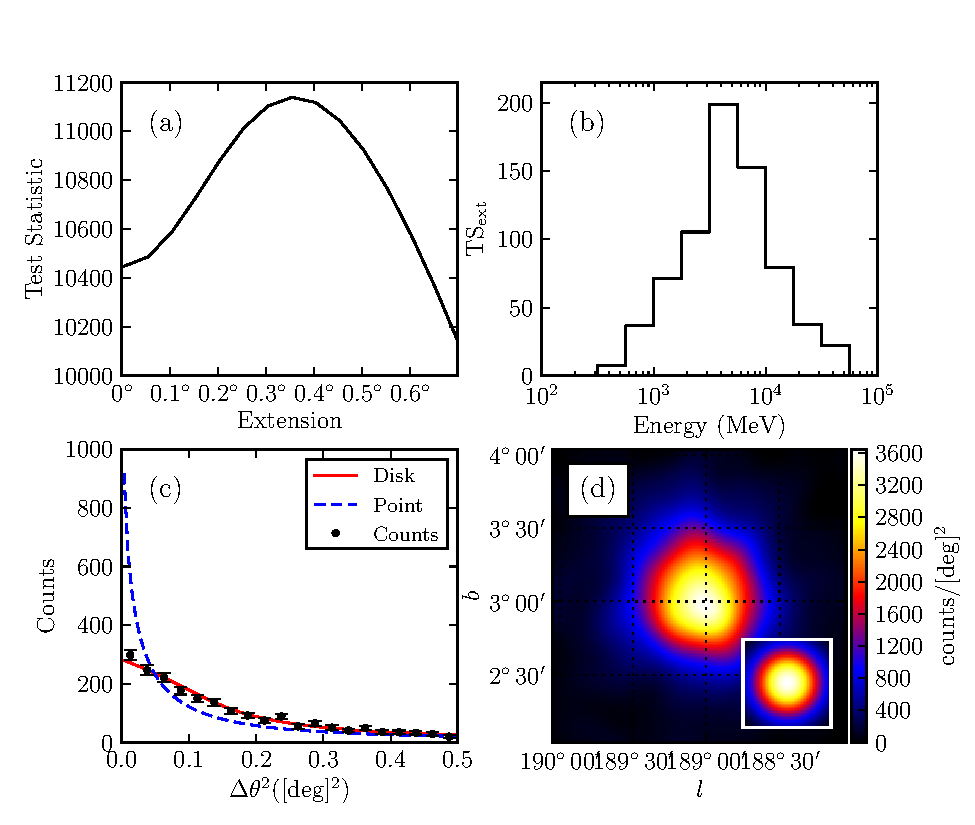
\includegraphics{ic443_plots/four_plots_ic443.pdf}
    % taken from /u/gl/lande/work/fermi/extended_catalog/2FGL/plots_for_paper/four_plots_ic443/v1/run.py
    \caption{
    Counts and test statistic profiles for the SNR IC443. (a) \ts
    vs. extension of the source. (b) \tsext for individual energy bands. (c)
    observed radial profile of counts in comparison to the expected profiles
    for a point source (blue) and a spatially extended source (red) . (d)
    smoothed count map after subtraction of the diffuse emission compared
    to the LAT PSF (inset).  Plots (a), (c), and (d) use only 1-100 \gev photons. 
    Plots (c) and (d)
    use only photons which converted in the front
    part of the detector and have an improved angular resolution.
    }
    \label{four_plots_ic443}
  \end{center}
\end{figure}

\clearpage
\begin{figure}
  \begin{center}
    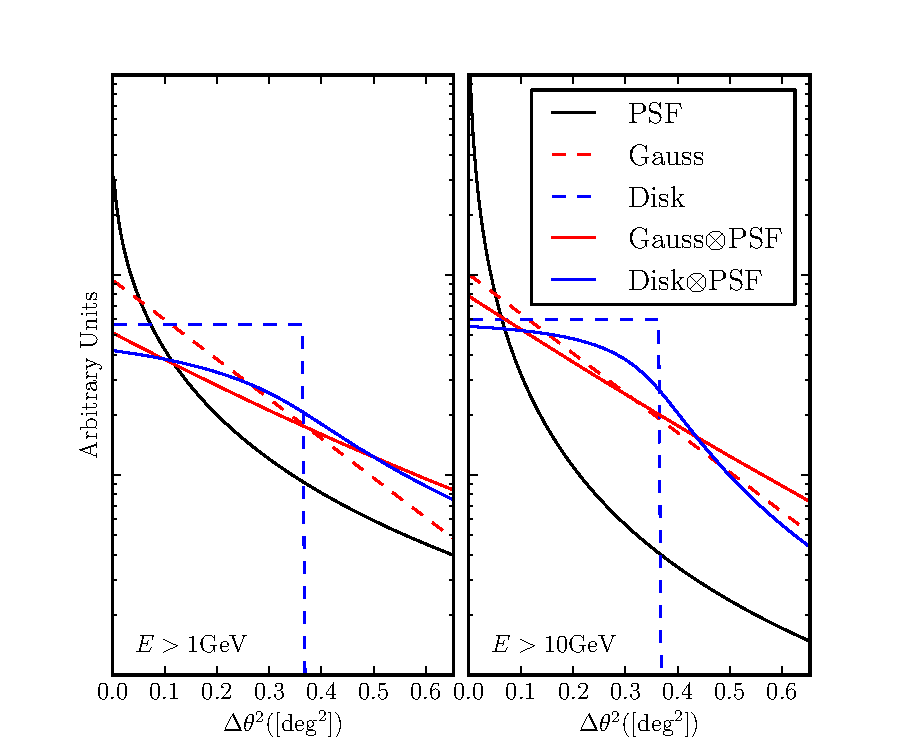
\includegraphics{mc_plots/compare_disk_gauss.pdf}
    % this plot came from /u/gl/lande/work/fermi/extended_catalog/2FGL/plots_for_paper/compare_disk_gauss/v2/compare_disk_gauss.pdf
    \end{center}
    \caption{
    A comparison of a Gaussian and disk like surface brightness profile
    of extended sources before and after convolving with the PSF for two
    energy ranges.  The black line is the PSF that would be observed
    for a power-law source of spectral index 2. The dashed red line
    is the brightness profile of a Gaussian with $\rsixeight=0.5\deg$.
    The dashed blue line is the brightness profile for a uniform disk
    with $\rsixeight=0.5\deg$.  The solid red and blue lines show the
    convolution of the Gaussian and uniform disk brightness profiles
    with the LAT PSF.
    }\label{compare_disk_gauss}
  \end{figure}


\clearpage
\begin{deluxetable}{rrrr}
\tabletypesize{\normalsize}
\tablecaption{Monte Carlo Validation Parameters
\label{ts_ext_num_sims}
}
\tablewidth{0pt}
\tablehead{

\colhead{Spectral Index}&
\colhead{Flux\tablenotemark{a}}&
\colhead{$N_\text{sims}$}&
\colhead{$\langle\ts\rangle$}
}

\startdata
      1.5 &          $10^{-6}$ &           31952 &  92862 \\
          &  $3\times 10^{-7}$ &           31962 &  22169 \\
          &          $10^{-7}$ &           31977 &   5806 \\
          &  $3\times 10^{-8}$ &           31991 &   1270 \\
          &          $10^{-8}$ &           31940 &    301 \\
          &  $3\times 10^{-9}$ &           30324 &     62 \\
      \hline
        2 &          $10^{-6}$ &           31872 &  22067 \\
          &  $3\times 10^{-7}$ &           31890 &   4898 \\
          &          $10^{-7}$ &           31858 &   1097 \\
          &  $3\times 10^{-8}$ &           31632 &    236 \\
          &          $10^{-8}$ &           27491 &    103 \\
      \hline
      2.5 &          $10^{-6}$ &           31822 &   4706 \\
          &  $3\times 10^{-7}$ &           31822 &    889 \\
          &          $10^{-7}$ &           31169 &    176 \\
          &  $3\times 10^{-8}$ &           21591 &     41 \\
      \hline                                                
      3   &          $10^{-6}$ &           31763 &    929 \\
          &  $3\times 10^{-7}$ &           31665 &    161 \\
          &          $10^{-7}$ &           19271 &     40 \\
\enddata

\tablenotetext{a}{Integral 1-100 \mev flux in units of $\ph/\cm^2/\sec$}

\tablecomments{
    the spectral models used in the Monte Carlo validation of \pointlike.
    For each model, the number of statistically independent simulations
    and the average value of \ts is tabulated.  The models spans
    representative spectral parameters.
}
\end{deluxetable}

\clearpage
\begin{figure}
  \begin{center}
    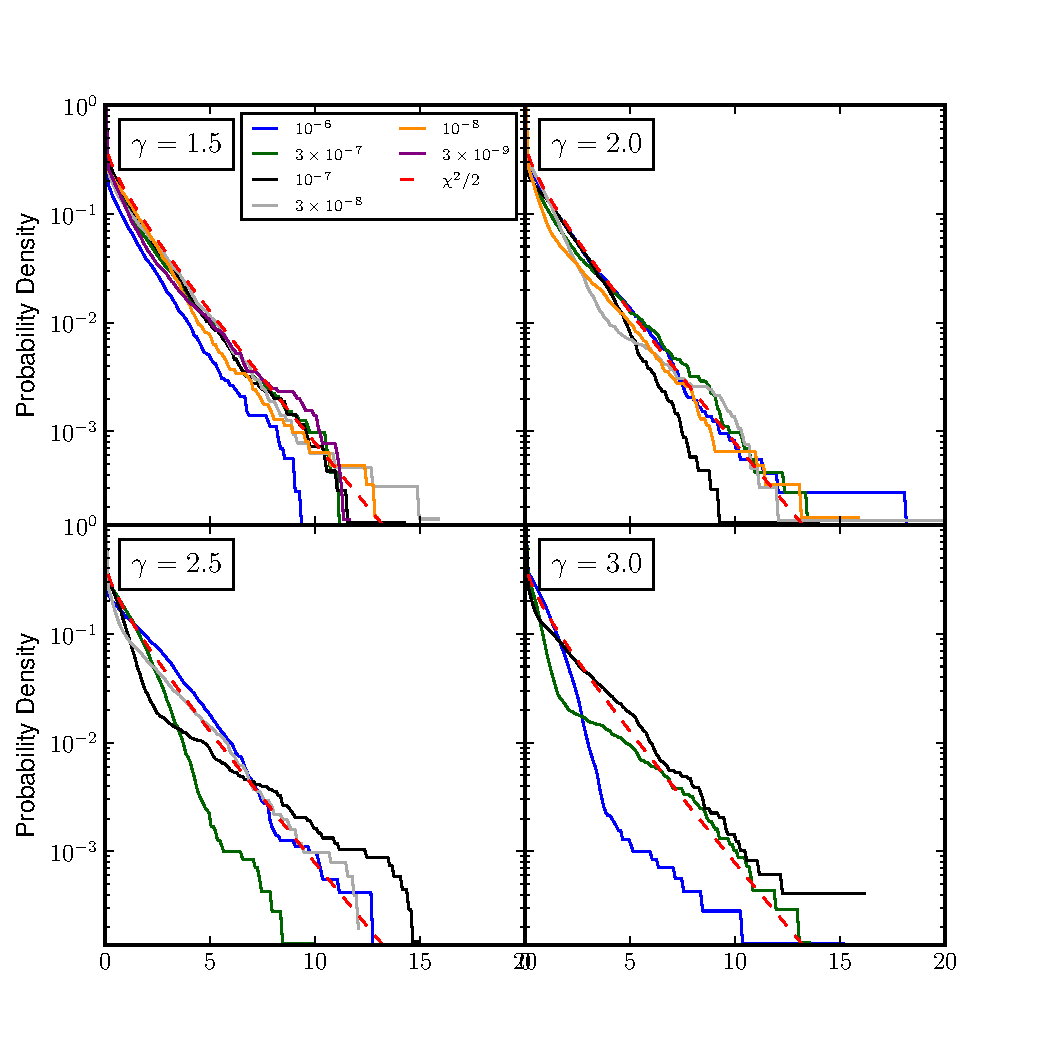
\includegraphics{mc_plots/ts_ext_emin_1000.pdf}
    % this plot came from /u/gl/lande/work/fermi/extended_catalog/monte_carlo/ts_ext/v3/plot.py
    % using data from /nfs/slac/g/ki/ki03/lande/extended_catalog/monte_carlo/ts_ext/v3_emin_1000/merged.hdf5
    \end{center}
    \caption{
    Distribution of the test statistic \tsext of a likelihood ratio
    test when fitting the extension of a point source.  The four plots
    represent simulated point sources of different spectral indices and
    the different colors represent point sources with different 100 \mev
    to 100 \gev integral fluxes.  The dashed red line is the cumulative
    density function of equation~\ref{ts_ext_distribution}.
    }\label{ts_ext_mc}
  \end{figure}

\clearpage

\begin{figure}
  \begin{center}
    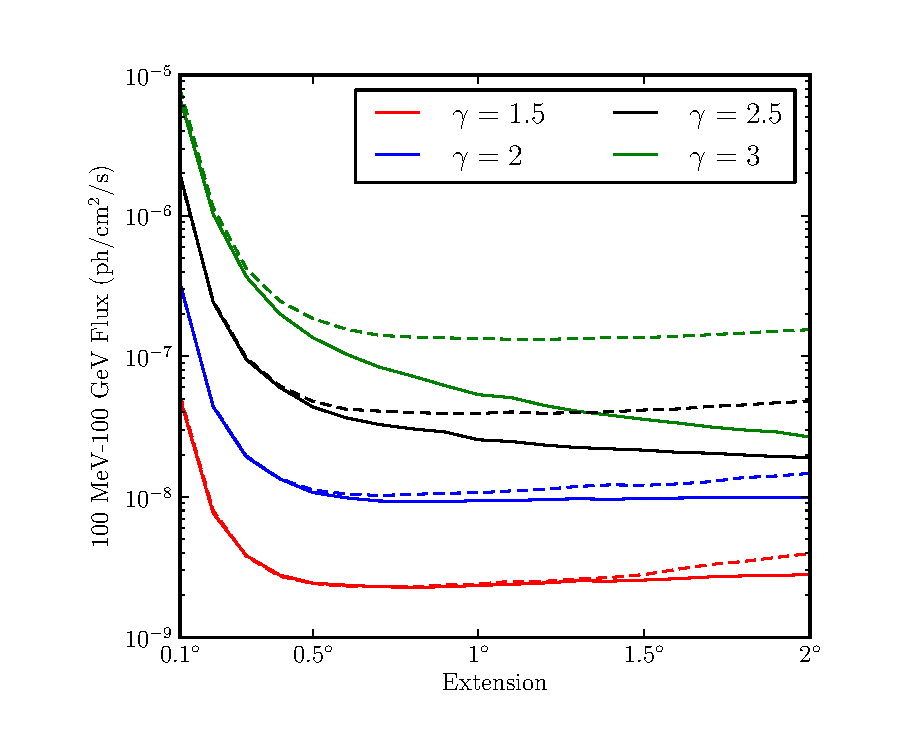
\includegraphics{mc_plots/index_sensitivity.pdf}
    % this plot came from /u/gl/lande/work/fermi/extended_catalog/monte_carlo/sensitivity/v12/plot/plot_vs_index.py
    \end{center}
    \caption{
    The detection threshold ($\langle\tsext\rangle=16$) to resolve a
    uniform disk extended source for a two-year exposure.  All sources
    have an assumed power-law spectrum and the different colors correspond
    to different simulated spectral indices.  The solid line is the
    detection threshold using photons with energy between 100 \mev and 100
    \gev while the dashed line is the threshold using 1-100 \gev photons.
    }\label{index_sensitivity}
  \end{figure}

\clearpage
\begin{figure}
  \begin{center}
    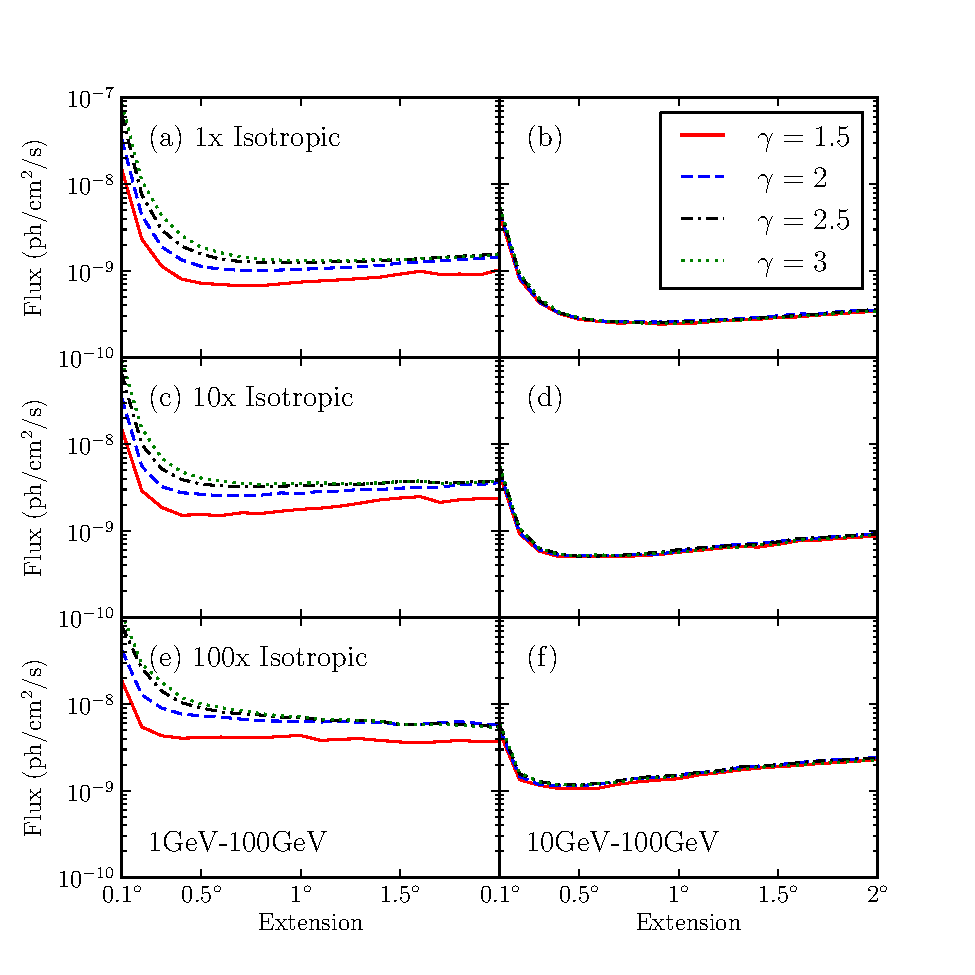
\includegraphics{mc_plots/all_sensitivity.pdf}
    % this plot came from /u/gl/lande/work/fermi/extended_catalog/monte_carlo/sensitivity/v12/plot/plot_all.py
    \end{center}
    \caption{the LAT detection threshold for four spectral indices and
    three background (1x, 10x, and 100x the Sreekumar-like isotropic
    spectrum) for a two-year exposure. The left plots are the detection
    threshold when using 1-100 \gev photons and the right plots are
    the detection threshold when using 10-100 \gev photons.  The flux
    is integrated only in the selected energy range.  Overlaid on this
    plot are the LAT detected extended sources placed by their nearby
    Galactic diffuse emission and color coded by their spectral index.
    The black point in plot (d) below the green line is MSH 15-52 which
    was found by our analysis to have $\tsext=6.5$.  
    }\label{all_sensitivity} 
  \end{figure}

  \clearpage
  \thispagestyle{empty}
\begin{deluxetable}{rrrrrrrrrrrrrrrrrrrrrrr}
\tabletypesize{\scriptsize}
\rotate
\tablewidth{0pt}
\tablecaption{Extension Detection Threshold
\label{all_sensitivity_table}
}
\tablehead{
\colhead{$\gamma$}&       
\colhead{BG}&
\colhead{$0.1$}&
\colhead{$0.2$}&
\colhead{$0.3$}&
\colhead{$0.4$}&
\colhead{$0.5$}&
\colhead{$0.6$}&
\colhead{$0.7$}&
\colhead{$0.8$}&
\colhead{$0.9$}&
\colhead{$1.0$}&
\colhead{$1.1$}&
\colhead{$1.2$}&
\colhead{$1.3$}&
\colhead{$1.4$}&
\colhead{$1.5$}&
\colhead{$1.6$}&
\colhead{$1.7$}&
\colhead{$1.8$}&
\colhead{$1.9$}&
\colhead{$2.0$}
}
\startdata
\multicolumn{22}{c}{E$>$1 \gev} \\
\hline
     1.5 &       x1 &      148.1 &       23.3 &       11.3 &        8.0 &        7.2 &        6.9 &        6.7 &        6.8 &        7.1 &        7.4 &        7.6 &        7.9 &        8.1 &        8.5 &        9.2 &        9.9 &        9.1 &        9.2 &        9.0 &       10.3 \\
         &      x10 &      148.4 &       29.0 &       18.7 &       15.2 &       15.4 &       15.0 &       16.1 &       16.0 &       16.8 &       17.7 &       18.2 &       19.3 &       20.9 &       22.5 &       23.8 &       24.8 &       21.3 &       22.8 &       23.4 &       23.7 \\
         &     x100 &      186.8 &       55.0 &       43.4 &       40.7 &       41.0 &       41.8 &       40.9 &       40.9 &       42.7 &       43.6 &       38.4 &       39.9 &       40.6 &       38.4 &       36.9 &       36.3 &       37.1 &       38.8 &       37.2 &       37.6 \\
       2 &       x1 &      328.4 &       43.4 &       18.9 &       13.4 &       11.2 &       10.4 &       10.2 &       10.2 &       10.2 &       10.4 &       10.7 &       10.9 &       11.2 &       11.5 &       12.4 &       12.6 &       13.0 &       13.4 &       14.0 &       14.4 \\
         &      x10 &      341.0 &       55.9 &       32.3 &       27.6 &       26.5 &       25.4 &       25.6 &       25.9 &       27.4 &       26.8 &       27.8 &       28.7 &       29.8 &       30.1 &       31.0 &       31.5 &       31.7 &       34.0 &       34.3 &       35.9 \\
         &     x100 &      420.5 &      128.3 &       90.2 &       77.3 &       73.3 &       70.8 &       67.5 &       64.3 &       64.2 &       64.1 &       62.8 &       63.6 &       61.7 &       61.9 &       58.4 &       59.0 &       61.4 &       63.3 &       60.1 &       58.1 \\
     2.5 &       x1 &      627.1 &       75.6 &       29.8 &       19.3 &       15.5 &       13.5 &       12.8 &       12.6 &       12.5 &       12.5 &       12.6 &       12.9 &       12.9 &       13.1 &       13.5 &       13.7 &       14.3 &       14.8 &       15.2 &       15.8 \\
         &      x10 &      638.9 &       99.1 &       52.1 &       39.1 &       34.6 &       33.0 &       32.5 &       32.5 &       32.8 &       33.2 &       34.1 &       34.3 &       34.5 &       35.1 &       36.6 &       36.9 &       35.5 &       36.0 &       36.5 &       37.3 \\
         &     x100 &      795.0 &      262.1 &      140.9 &      104.3 &       90.4 &       81.2 &       77.2 &       75.1 &       69.7 &       70.9 &       66.5 &       65.6 &       64.9 &       64.0 &       58.9 &       58.1 &       60.2 &       58.4 &       57.5 &       55.8 \\
       3 &       x1 &      841.5 &      110.6 &       43.2 &       25.5 &       18.7 &       16.1 &       14.4 &       13.6 &       13.3 &       13.2 &       13.1 &       13.1 &       13.4 &       13.6 &       13.5 &       13.8 &       14.2 &       14.4 &       14.8 &       15.4 \\
         &      x10 &      921.6 &      151.3 &       69.1 &       47.8 &       40.7 &       37.1 &       35.5 &       34.5 &       35.1 &       35.5 &       35.3 &       35.3 &       35.4 &       35.5 &       36.8 &       37.6 &       35.3 &       35.4 &       36.3 &       36.6 \\
         &     x100 &     1124.1 &      282.9 &      181.1 &      119.8 &      100.7 &       91.1 &       84.3 &       77.9 &       73.3 &       71.8 &       67.6 &       66.4 &       65.5 &       63.9 &       59.0 &       58.6 &       58.8 &       57.5 &       55.4 &       54.4 \\
\cutinhead{E$>$10 \gev}
     1.5 &       x1 &       44.6 &        8.0 &        4.3 &        3.2 &        2.7 &        2.6 &        2.5 &        2.5 &        2.4 &        2.5 &        2.5 &        2.6 &        2.7 &        2.8 &        2.9 &        2.9 &        3.1 &        3.2 &        3.3 &        3.4 \\
         &      x10 &       45.2 &        9.2 &        5.8 &        5.0 &        4.9 &        4.9 &        5.0 &        5.2 &        5.3 &        5.7 &        5.9 &        6.3 &        6.6 &        6.5 &        6.8 &        7.6 &        7.8 &        8.2 &        8.5 &        8.7 \\
         &     x100 &       47.3 &       13.4 &       11.6 &       10.6 &       10.8 &       10.8 &       12.0 &       12.7 &       13.2 &       13.7 &       15.3 &       16.1 &       17.2 &       18.2 &       18.9 &       19.5 &       20.4 &       21.0 &       21.7 &       22.9 \\
       2 &       x1 &       49.7 &        8.4 &        4.4 &        3.3 &        2.8 &        2.6 &        2.6 &        2.6 &        2.6 &        2.6 &        2.7 &        2.7 &        2.8 &        2.9 &        3.0 &        3.2 &        3.2 &        3.4 &        3.5 &        3.5 \\
         &      x10 &       48.6 &        9.5 &        6.0 &        5.2 &        5.0 &        5.2 &        5.2 &        5.3 &        5.4 &        5.8 &        6.4 &        6.6 &        7.0 &        7.1 &        7.5 &        8.0 &        8.3 &        8.6 &        9.0 &        9.2 \\
         &     x100 &       51.8 &       14.7 &       11.8 &       11.5 &       11.5 &       11.9 &       13.2 &       14.0 &       14.3 &       15.3 &       16.2 &       16.9 &       18.4 &       19.2 &       19.8 &       21.0 &       22.0 &       22.8 &       23.2 &       24.3 \\
     2.5 &       x1 &       53.1 &        9.1 &        4.5 &        3.3 &        2.8 &        2.7 &        2.6 &        2.5 &        2.5 &        2.6 &        2.7 &        2.7 &        2.8 &        2.8 &        2.9 &        3.1 &        3.2 &        3.3 &        3.5 &        3.6 \\
         &      x10 &       53.7 &       10.5 &        6.3 &        5.4 &        5.1 &        5.1 &        5.3 &        5.4 &        5.7 &        6.0 &        6.3 &        6.6 &        6.8 &        6.9 &        7.5 &        8.1 &        8.3 &        8.6 &        8.9 &        9.2 \\
         &     x100 &       57.0 &       15.6 &       12.7 &       11.9 &       11.8 &       12.2 &       13.1 &       14.3 &       14.6 &       15.2 &       16.3 &       17.0 &       18.8 &       19.2 &       19.9 &       21.0 &       21.9 &       22.3 &       23.3 &       23.7 \\
       3 &       x1 &       55.5 &        9.4 &        4.8 &        3.4 &        2.9 &        2.7 &        2.6 &        2.5 &        2.5 &        2.5 &        2.6 &        2.7 &        2.7 &        2.8 &        2.9 &        3.0 &        3.1 &        3.2 &        3.4 &        3.4 \\
         &      x10 &       56.0 &       10.5 &        6.2 &        5.3 &        5.1 &        5.1 &        5.1 &        5.3 &        5.5 &        5.7 &        5.9 &        6.4 &        6.4 &        6.6 &        7.0 &        7.8 &        8.0 &        8.3 &        8.6 &        8.9 \\
         &     x100 &       60.3 &       16.2 &       12.7 &       11.7 &       11.8 &       12.2 &       12.6 &       13.8 &       14.2 &       14.6 &       15.8 &       16.5 &       17.6 &       18.5 &       19.4 &       19.8 &       20.7 &       21.0 &       21.8 &       22.5 \\
\enddata
\tablecomments{
      The detection threshold to resolve a uniform disk spatially extended
      sources using two years of data for sources of varying energy
      ranges, spectral indices, and background levels.  The extended
      sources were simulated against a Sreekumar-like isotropic spectrum
      and the second column is the factor that the simulated background
      was scaled by. The remaining columns are varying sizes of the source
      in degrees assuming a uniform surface brightness. The table quotes
      integral fluxes in the analyzed energy range (1-100 \gev or 10-100
      \gev) in units of $10^{-10}\ph/\cm^2/\sec$.
      }
\end{deluxetable}




\begin{figure}
  \begin{center}
    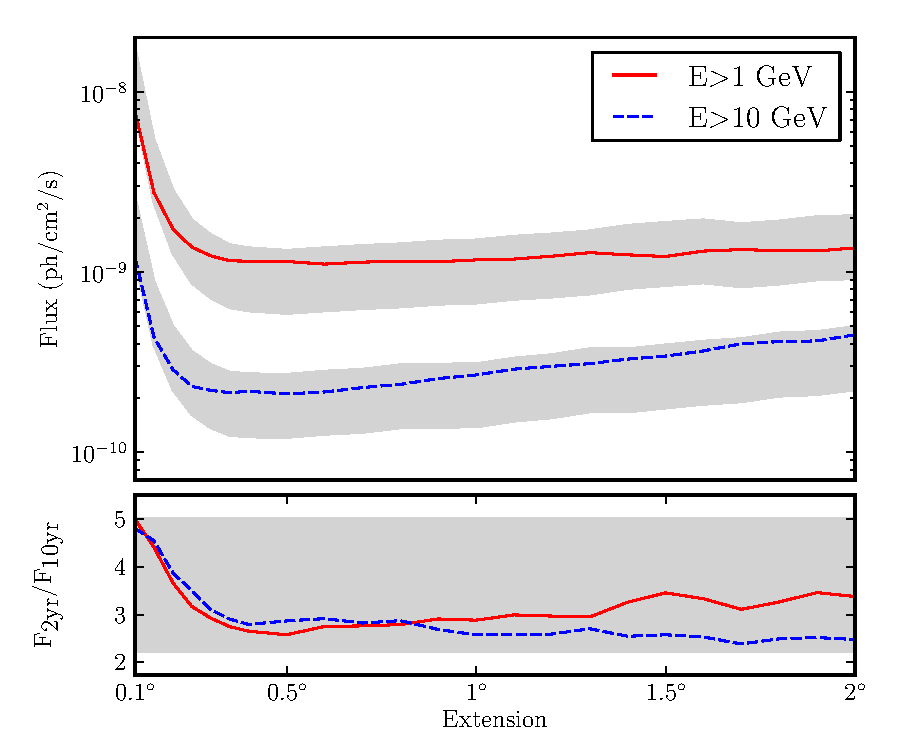
\includegraphics{mc_plots/time_sensitivity.pdf}
    % this plot came from /u/gl/lande/work/fermi/extended_catalog/monte_carlo/sensitivity/v12/plot/plot_vs_time.py
    \end{center}
    \caption{
    The LAT's projected detection theshold to extension after 10 years for a power-law
    source of spectral index 2 against 10 times the isotropic background
    in the energy range from 1-100 \gev (solid red) and 10-100 \gev
    (dashed blue). The solid gray region is the 
    detection threshold assuming the sensitivity improves from the 2
    year threshold by $\sqrt{\text{t}}$ (top edge) and linearly with
    time (bottom edge).  The lower plot shows the factor increase in
    sensitivity.  For small extended sources, our detection threshold
    improves by a factor better than $\sqrt{\text{t}}$. 
    }\label{time_sensitivity}
  \end{figure}


\clearpage
\begin{figure}
  \begin{center}
    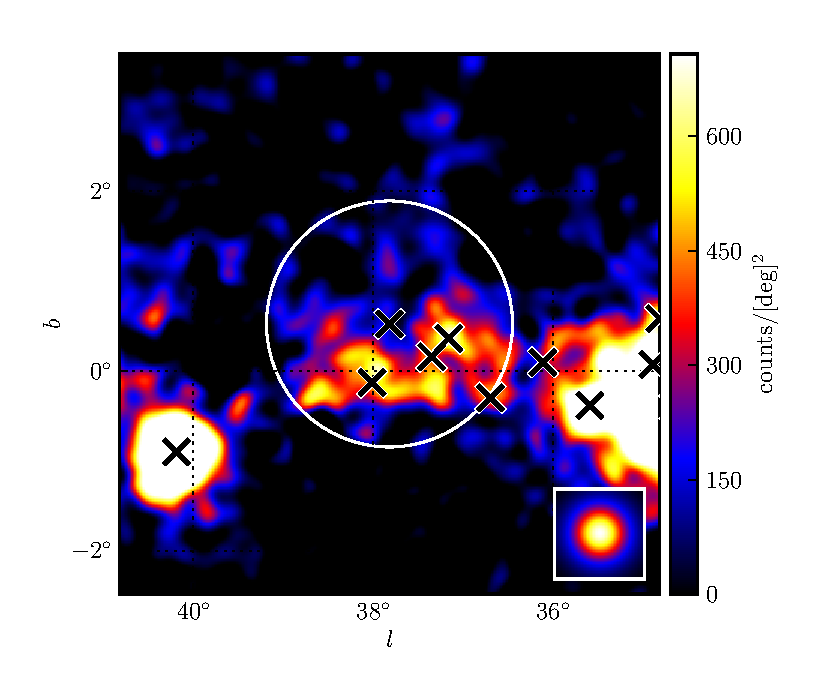
\includegraphics{source_plots/example_bad_fit.pdf}
    % taken from /u/gl/lande/work/fermi/extended_catalog/2FGL/plots_for_paper/example_bad_fit/v3/run.py
    \caption{
    A Diffuse emission subtracted 1-100 \gev counts map of the region
    around 2FGL\,J1856.2+0450c smoothed by a 0.1\deg Gaussian kernel. The
    red cross and circle are the center and size of the best fit radially
    symmetric source with a uniform intensity profile. The result is
    statistically significant, but the extension encompasses many catalog
    sources and the emission does not look to be uniform. Instead,
    this source is probably fitting large-scale diffuse residual
    features. Although the fit is statistically significant, it likely
    corresponds to residual features of inaccurately modeled diffuse
    emission picked up by the fit.  We manually discard candidates that
    appear like this.
    }
    \label{example_bad_fit}
  \end{center}
\end{figure}

\begin{figure}
  \begin{center}
  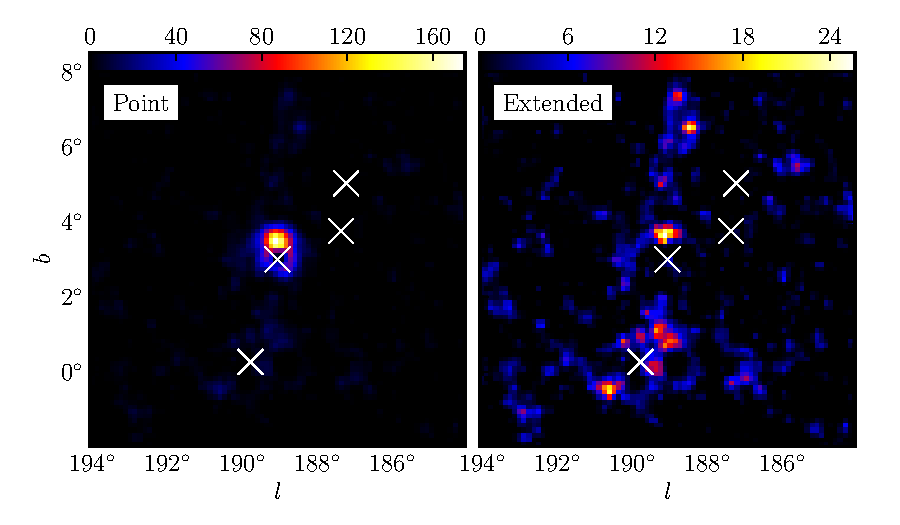
\includegraphics{ic443_plots/res_tsmap_ic443.pdf}
  % plot from /u/gl/lande/work/fermi/extended_catalog/2FGL/plots_for_paper/res_tsmap_ic443/v1

  \caption{
  A test statistic map generated for the region around supernova
  remnant IC443 using 1-100 \gev photons.  (a) test statistic map after
  subtracting IC443 modeled as a point source. (b) same as (a), but
  IC443 modeled as extended source. Crosses represent sources included
  in the model of the region.  Such maps were generated for all extended
  source candidates.}
  \label{res_tsmaps}
  \end{center}
\end{figure}


\begin{deluxetable}{lrrrrrrrr}
\rotate
\tabletypesize{\footnotesize}
\tablewidth{0pt}
\tablecaption{Extension fit for the twelve extended sources included in 2FGL
\label{known_extended_sources}
}
\tablehead{
\colhead{Name}&
\colhead{\glon\tablenotemark{a}}&
\colhead{\glat\tablenotemark{a}}&
\colhead{$\sigma$\tablenotemark{a}}&
\colhead{\ts}&
\colhead{\tsext}&
\colhead{Pos Err\tablenotemark{a}}&
\colhead{Flux\tablenotemark{b}}&
\colhead{Index}
}

\startdata
\multicolumn{9}{c}{E$>$1 \gev} \\
\hline
SMC                  &     302.68 &     -44.81 & $  1.75 \pm   0.07 \pm   0.02 $ &       94.8 &       67.4 &   0.12 & $    3.3 \pm     0.4$ & $   2.41 \pm    0.17$  \\
LMC                  &     279.10 &     -32.61 & $  1.74 \pm   0.05 \pm   0.13 $ &     1101.3 &      860.5 &   0.05 & $   15.5 \pm     0.6$ & $   2.48 \pm    0.06$  \\
IC443                &     189.05 &       3.04 & $  0.36 \pm   0.01 \pm   0.04 $ &    10719.8 &      510.4 &   0.01 & $   64.8 \pm     1.2$ & $   2.23 \pm    0.02$  \\
Vela X               &     263.34 &      -3.11 & $                         0.88$ &            &            &        &                       &                        \\
Centarus A           &     309.52 &      19.42 &                     $\approx10$ &            &            &        &                       &                        \\
W28                  &       6.50 &      -0.27 & $  0.43 \pm   0.02 \pm   0.03 $ &     1324.8 &      177.4 &   0.01 & $   58.0 \pm     1.8$ & $   2.63 \pm    0.03$  \\
W30                  &       8.61 &      -0.20 & $  0.36 \pm   0.02 \pm   0.02 $ &      465.4 &       73.3 &   0.02 & $   30.7 \pm     1.6$ & $   2.59 \pm    0.04$  \\
W44                  &      34.69 &      -0.38 & $  0.36 \pm   0.01 \pm   0.02 $ &     1903.3 &      217.7 &   0.01 & $   73.6 \pm     1.8$ & $   2.68 \pm    0.02$  \\
W51C                 &      49.13 &      -0.45 & $  0.28 \pm   0.02 \pm   0.05 $ &     1819.5 &      115.7 &   0.01 & $   39.3 \pm     1.3$ & $   2.35 \pm    0.03$  \\
Cygnus Loop          &      74.22 &      -8.46 & $  1.72 \pm   0.05 \pm   0.07 $ &      356.5 &      356.5 &   0.06 & $   11.1 \pm     0.7$ & $   2.53 \pm    0.11$  \\
\cutinhead{E$>$10 \gev}
MSH 15-52            &     320.38 &      -1.22 & $  0.20 \pm   0.04 \pm   0.03 $ &       76.2 &        6.5 &   0.03 & $    0.6 \pm     0.7$ & $   2.27 \pm    0.73$  \\
HESS J1825-137       &      17.56 &      -0.46 & $  0.65 \pm   0.03 \pm   0.01 $ &       83.6 &       55.9 &   0.05 & $    1.8 \pm     0.2$ & $   1.74 \pm    0.19$  \\
\enddata

\tablenotetext{a}{in degrees.}
\tablenotetext{b}{
integrated in the fit energy range (either 1-100 \gev or 10-100 \gev)
in units of $10^{-9}\ph/\cm^2/\sec$.
}

\tablecomments{
All sources were fit using a spatial model assuming a uniform radially
symmetric intensity distribution. \glon and \glat are Galactic longitude
and latitude of the best fit extended source respectively.  The first
error on $\sigma$ is statistical and the second is systematic (see
section~\ref{systematic_errors_on_extension}).  Pos Err is the error on
the position of the source.  Vela X and the Centarus A Lobes were
not fit by our analysis but are include for completeness.
}
\end{deluxetable}


\clearpage
\begin{figure}
  \begin{center}
    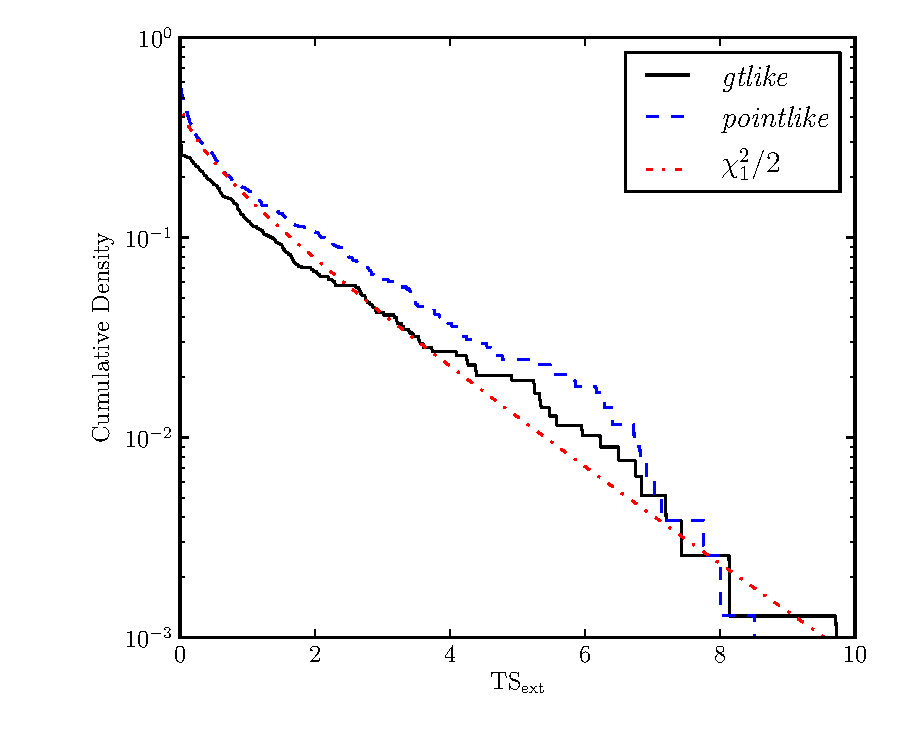
\includegraphics{source_plots/agn.pdf}
    % this plot came from /u/gl/lande/work/fermi/extended_catalog/2FGL/agn/v2/agn.py
    \end{center}
    \caption{The cumulative density of \tsext for 783 of the clean
    AGN in 2LAC which are significant above 1 \gev.  AGNs are too far
    and too small to be resolved by the LAT. Therefore, the cumulative
    density of $\tsext$ is expected to follow a $\chi^2/2$ distribution
    (equation~\ref{ts_ext_distribution}).     
    }\label{agn_ts_ext}
  \end{figure}


  % 1FGL J1628.6-2419c - P72Y2516         - 2FGL J1627.0-2425c
  % 1FGL J0823.3-4248  - P72Y1212         - 2FGL J0823.0-4246
  % 1FGL J1614.7-5138c - P72Y2473         - 2FGL J1615.2-5138
  % 1FGL J1632.9-4802c - P72Y2540         - 2FGL J1632.4-4753c
  % 1FGL J2020.0+4049  - P72Y3281         - 2FGL J2021.5+4026
  % 1FGL J1837.5-0659c - P72Y2974         - 2FGL J1837.3-0700c
  % N/A                - P72Y1287         - 2FGL J0851.7-4635


\clearpage
\thispagestyle{empty}
\begin{deluxetable}{lrrrrrrrrr}
\tabletypesize{\small}
\rotate
\tablewidth{0pt}
\tablecaption{Extension fit for the nine new extended sources
\label{new_ext_srcs_table}
}
\tablehead{
\colhead{Name}&
\colhead{\glon}&
\colhead{\glat}&
\colhead{$\sigma$}&
\colhead{\ts}&
\colhead{\tsext}&
\colhead{Pos Err}&
\colhead{Flux}&
\colhead{Index}&
\colhead{Counterpart}
}

\startdata
\multicolumn{10}{c}{E$>$1 \gev} \\
\hline
2FGL\,J0823.0-4246   &     260.32 &      -3.28 & $  0.37 \pm   0.03 \pm   0.02 $ &      320.9 &       46.3 &   0.02 & $    8.5 \pm     0.7$ & $   2.20 \pm    0.09$ &             Puppis A \\
2FGL\,J1627.0-2425c  &     353.08 &      16.78 & $  0.41 \pm   0.05 \pm   0.02 $ &      144.5 &       31.1 &   0.04 & $    6.5 \pm     0.6$ & $   2.49 \pm    0.14$ &            Ophiuchus \\
2FGL\,J1712.4-3941   &     347.25 &      -0.54 & $  0.56 \pm   0.04 \pm   0.01 $ &       75.0 &       39.6 &   0.05 & $    4.2 \pm     0.9$ & $   1.47 \pm    0.12$ &     RX\,J1713.7-3946 \\
\cutinhead{E$>$10 \gev}
2FGL\,J0851.7-4635   &     266.29 &      -1.43 & $  1.13 \pm   0.08 \pm   0.05 $ &      116.1 &       87.2 &   0.07 & $    1.3 \pm     0.2$ & $   1.76 \pm    0.21$ &             Vela Jr. \\
2FGL\,J1615.0-5051   &     332.38 &      -0.14 & $  0.33 \pm   0.04 \pm   0.01 $ &       53.4 &       16.3 &   0.04 & $    1.1 \pm     0.2$ & $   2.24 \pm    0.28$ &      HESS\,J1616-508 \\
2FGL\,J1615.2-5138   &     331.66 &      -0.66 & $  0.42 \pm   0.03 \pm   0.01 $ &       76.6 &       48.0 &   0.05 & $    1.2 \pm     0.2$ & $   1.77 \pm    0.24$ &      HESS\,J1614-518 \\
2FGL\,J1632.4-4753c  &     336.41 &       0.22 & $  0.44 \pm   0.04 \pm   0.03 $ &      127.8 &       64.5 &   0.04 & $    1.9 \pm     0.2$ & $   2.29 \pm    0.21$ &      HESS\,J1632-478 \\
2FGL\,J1837.3-0700c  &      25.08 &       0.13 & $  0.35 \pm   0.08 \pm   0.03 $ &       46.2 &       18.8 &   0.07 & $    1.0 \pm     0.2$ & $   1.63 \pm    0.29$ &      HESS\,J1837-069 \\
2FGL\,J2021.5+4026   &      78.18 &       2.19 & $  0.59 \pm   0.03 \pm   0.02 $ &      222.2 &      116.4 &   0.04 & $    1.8 \pm     0.2$ & $   2.31 \pm    0.19$ &       $\gamma$ Cygni \\
\enddata

\tablecomments{
    The columns in this table
    are equivalent to the columns in table~\ref{known_extended_sources}.
}
\end{deluxetable}



\clearpage
\thispagestyle{empty}
\begin{deluxetable}{lrrrrrrrrrr}
  \rotate
  \tablewidth{0pt}
  \tablecaption{Dual localization, alternative PSF, and alternative diffuse results
  \label{alt_diff_model_results}
  }
  \tablehead{
  \colhead{Name}&
  \colhead{$\ts_\pointlike$}&
  \colhead{$\ts_\gtlike$}&
  \colhead{$\ts_\altdiff$}&
  \colhead{$\tsext_\pointlike$}&
  \colhead{$\tsext_\gtlike$}&
  \colhead{$\tsext_\altdiff$}&
  \colhead{$\sigma$\tablenotemark{a}}&
  \colhead{$\sigma_\altdiff$\tablenotemark{a}}&
  \colhead{$\sigma_\altpsf$\tablenotemark{a}}&
  \colhead{$\tsinc$}
  }
  \startdata
  \multicolumn{11}{c}{E$>$1 \gev} \\
  \hline
  2FGL\,J0823.0-4246   &                350.9 &                320.9 &                352.5 &                 66.0 &                 46.3 &                 53.6 &                 0.37 &                 0.39 &                 0.38 &                 22.1 \\
  2FGL\,J1627.0-2425c  &                170.2 &                144.5 &                112.6 &                 43.9 &                 31.1 &                 23.9 &                 0.41 &                 0.40 &                 0.39 &                 20.0 \\
  2FGL\,J1712.4-3941   &                 80.9 &                 75.0 &                 43.4 &                 47.4 &                 39.6 &                 22.2 &                 0.56 &                 0.56 &                 0.54 &                  6.4 \\
  \cutinhead{E$>$10 \gev}
  2FGL\,J0851.7-4635   &                116.7 &                116.1 &                122.3 &                 87.1 &                 87.2 &                 90.4 &                 1.13 &                 1.16 &                 1.17 &                 16.1 \\
  2FGL\,J1615.0-5051   &                 52.4 &                 53.4 &                 55.6 &                 17.5 &                 16.3 &                 17.4 &                 0.33 &                 0.32 &                 0.32 &                 11.9 \\
  2FGL\,J1615.2-5138   &                 76.3 &                 76.6 &                 86.3 &                 44.0 &                 48.0 &                 52.6 &                 0.42 &                 0.43 &                 0.43 &                 37.0 \\
  2FGL\,J1632.4-4753c  &                126.6 &                127.8 &                120.7 &                 63.9 &                 64.5 &                 64.1 &                 0.44 &                 0.44 &                 0.47 &                 40.6 \\
  2FGL\,J1837.3-0700c  &                 45.4 &                 46.2 &                 39.0 &                 18.5 &                 18.8 &                 16.6 &                 0.35 &                 0.34 &                 0.38 &                 12.6 \\
  2FGL\,J2021.5+4026   &                234.3 &                222.2 &                235.6 &                135.9 &                116.4 &                121.4 &                 0.59 &                 0.60 &                 0.60 &                 24.3 \\
  \enddata

\tablenotetext{a}{in degrees.}

\tablecomments{
$\ts_\pointlike$, $\ts_\gtlike$, and $\ts_\altdiff$ are the test
statistic values from \pointlike, \gtlike, and with the alternate
diffuse model respectively.  $\tsext_\pointlike$, $\tsext_\gtlike$,
and $\tsext_\altdiff$ are the test statistic values of the extension
test from \pointlike, \gtlike, and with the alternate diffuse
model respectively.  $\sigma$, $\sigma_\altdiff$, and $\sigma_\altpsf$
are the fit extension with the standard analysis,
alternate diffuse model, and alternate PSF respectively.  \tsinc is
the test statistic for the two point source test.
}
\end{deluxetable}


\begin{figure}
  \begin{center}
    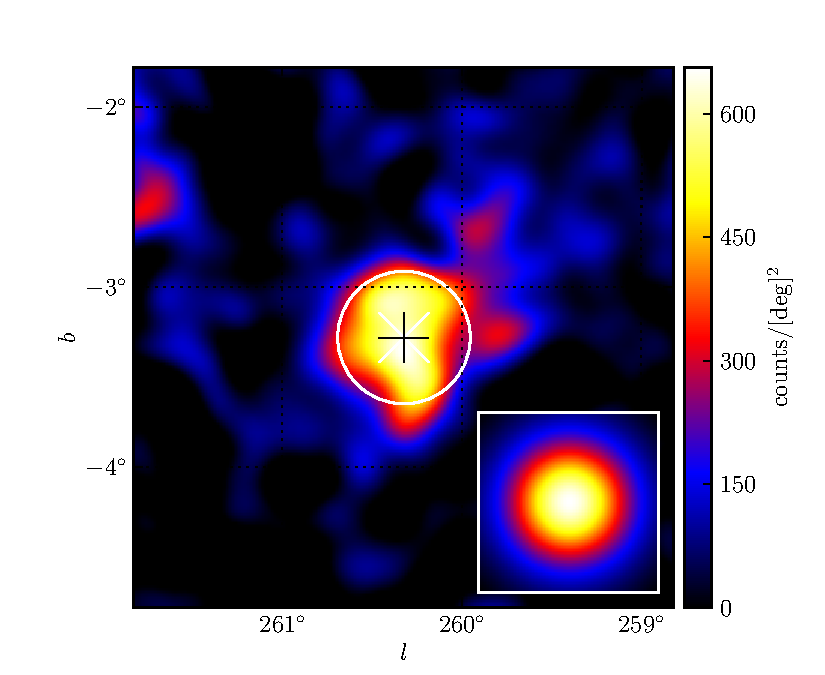
\includegraphics[type=pdf,ext=.pdf,read=.pdf]{source_plots/source_1FGL_J0823.3-4248}
  \end{center}
  % this plot came from 
  % /u/gl/lande/work/fermi/extended_catalog/2FGL/plots_for_paper/source_plots/1FGL_J0823.3-4248/v2/source_1FGL_J0823.3-4248.pdf
  \caption{A Diffuse emission subtracted 1-100
  \gev counts map of the region around 2FGL\,J0823.0-4246 smoothed
  by a 0.1\deg Gaussian kernel.  The red star is the catalog position
  of this source.  The red cross and circle are the best fit position
  and extension of this source assuming a radially symmetric uniform
  surface brightness.  The two green stars are the positions of the
  sources 2FGL\,J0823.4-4305 and 2FGL\,J0821.0-4254 which were removed
  because they are part of the extended source.  The lower right inset
  is the model predicted emission from a point source with the same
  spectrum as 2FGL\,J0823.4-4305 smoothed by the same Gaussian kernel.
  This source is spatially coincident with the Puppis A SNR. The
  light blue contours correspond to the X-ray image of Puppis A observed by 
  \rosat
  \citep{rosat_puppis_a}. 
  }\label{1FGL_J0823.3-4248}
\end{figure}

\begin{figure}
  \begin{center}
    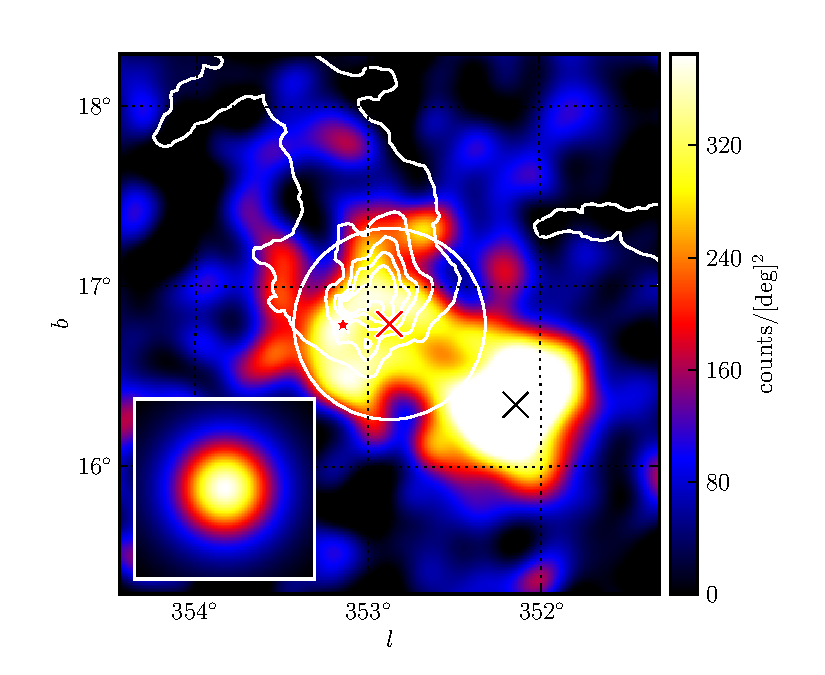
\includegraphics[type=pdf,ext=.pdf,read=.pdf]{source_plots/source_1FGL_J1628.6-2419c}
  \end{center}
  % this plot came from 
  % /u/gl/lande/work/fermi/extended_catalog/2FGL/plots_for_paper/source_plots/1FGL_J1628.6-2419c/v2/run.py
  \caption{
  A Diffuse emission subtracted 1-100 \gev counts
  map of (a) the region around 2FGL\,J1627.0-2425 smoothed by a 0.1\deg
  Gaussian kernel (b) also the emission from the background source 
  2FGL\,J1625.7-2526 subtracted.  The red star is the catalog's
  position of this source.  The red cross and circle are the best
  position and extension of this source assuming a radially symmetric
  uniform surface brightness.  The left contours correspond to the
  100 micrometer image observed by IRAS \citep{iras_rho_ophiuci} and the right
  contours correspond to CO emission \citep{co_rho_ophiuci}.
  \todo[inline]{Rewrite CO contours based upon descritipon
  of CO contours in Cygnus Loop paper
  http://arxiv.org/pdf/1108.1833v2
  }
  }\label{1FGL_J1628.6-2419c}
\end{figure}

\begin{figure}
  \begin{center}
    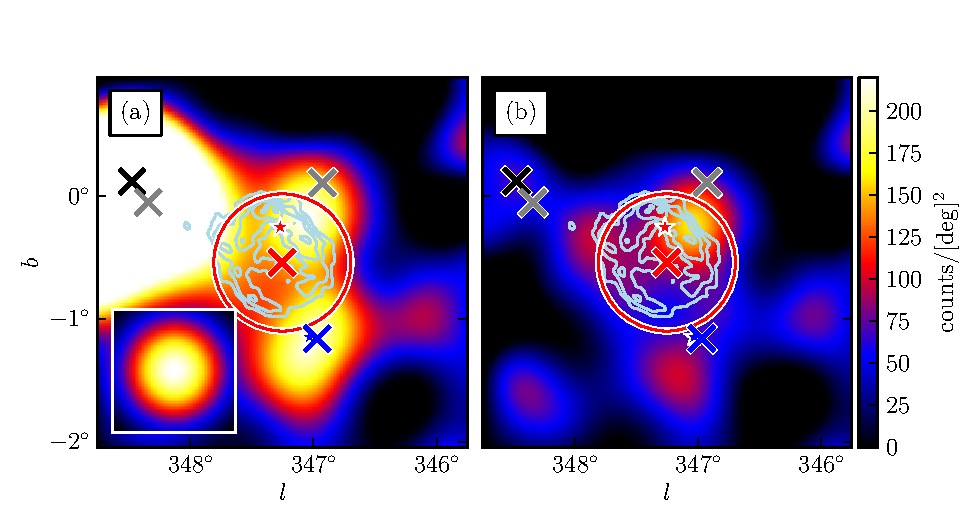
\includegraphics[type=pdf,ext=.pdf,read=.pdf]{source_plots/source_RX_J1713.7-3946}
    % this plot came from
  % /u/gl/lande/work/fermi/extended_catalog/2FGL/plots_for_paper/source_plots/RX_J1713.7-3946/v6/run.py
  \end{center}
  \caption{A Diffuse emission subtracted 1-100 \gev
  counts map of (a) the region around 2FGL\,J1712.4-3941 smoothed by
  a 0.25\deg Gaussian kernel and (b) also the emission 
  from the background sources subtracted.
  This source is spatially
  coincident with RX J1713.7-3946 was was recently reported by
  \citep{rx_j1713_lat}.  The light blue contours correspond to the \tev image
  observed by H.E.S.S. \citep{rx_j1713_hess}.  The region was analyzed
  with the same background model as \citep{rx_j1713_lat}.  Source A (blue
  cross) is spatially coincident with 2FGL\,J1715.4-4024c (blue star).
  The gray crosses represent from left to right the position of source B
  and C which were added to the background model. 
  }\label{2FGL_J1712.4-3941}
\end{figure}



\begin{figure}
  \begin{center}
    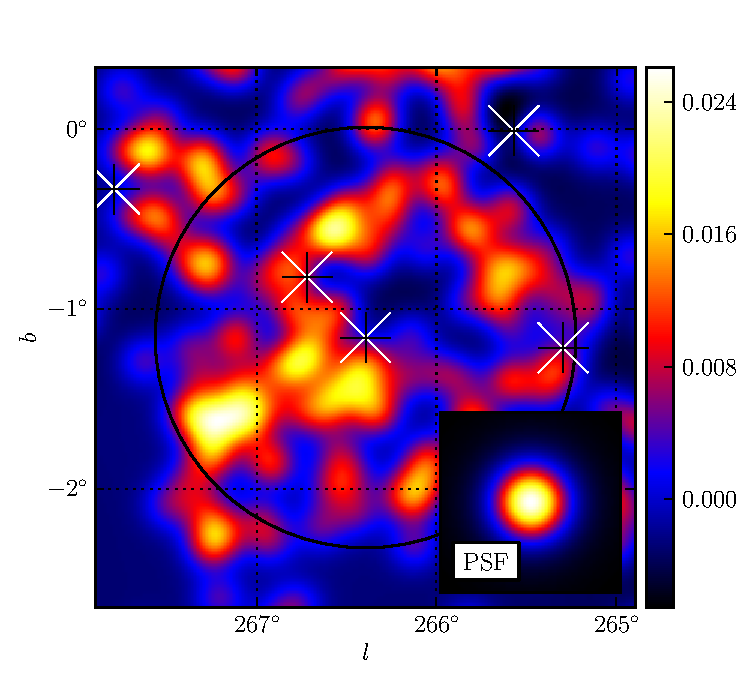
\includegraphics[type=pdf,ext=.pdf,read=.pdf]{source_plots/source_Vela_Jr}
  \end{center}
  % this plot came from 
  % /u/gl/lande/work/fermi/extended_catalog/2FGL/plots_for_paper/source_plots/Vela_Jr/v2/source_Vela_Jr.pdf
  \caption{A Diffuse emission subtracted 10-100
  \gev counts map of the region around 2FGL\,J0851.7-4635 smoothed
  by a 0.25\deg Gaussian kernel. The red star is the catalog position of this source.  The red cross
  and circle are the best fit position and extension of the source
  assuming a radially
  symmetric uniform surface brightness.  The inner three green stars
  are (from left to right) 2FGL\,J0853.5-4711, 2FGL\,J0855.4-4625,
  and 2FGL\,J0848.5-4535 which were removed because they are part of
  the extended source.  The farther away green stars are (from left to
  right) 2FGL\,J0901.7-4655 and 2FGL\,J0858.0-4815 which were removed
  because they were not significant above 10 \gev.  The blue cross
  is the relocalized position of 2FGL\,J0854.7-4501.  This extended
  source is spatially coincident with the Vela Jr SNR.  The light
  blue contours correspond to the \tev image of Vela Jr. observed by H.E.S.S
  \citep{vela_jr_hess}.
  }\label{Vela_Jr}
\end{figure}

\begin{figure}
  \begin{center}
    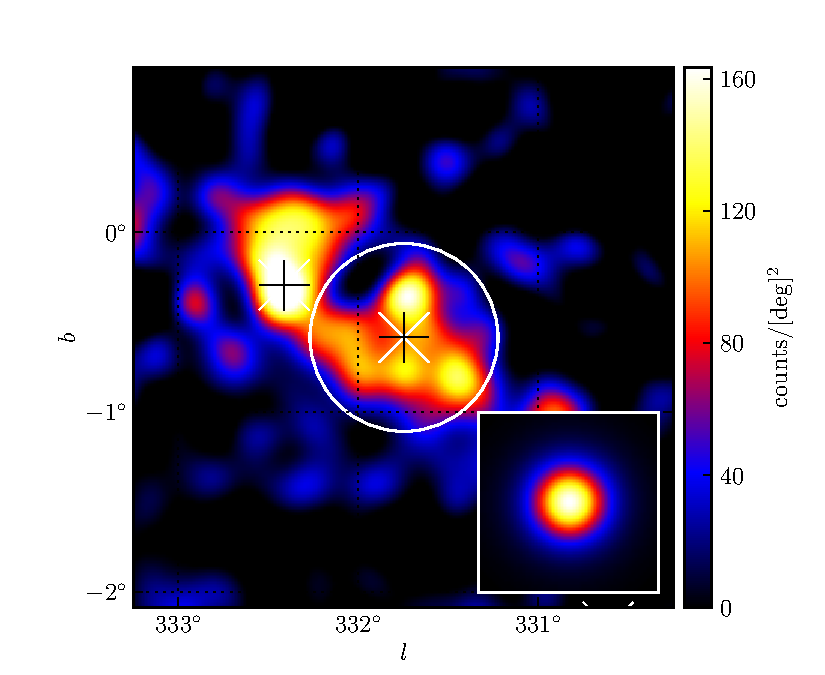
\includegraphics[type=pdf,ext=.pdf,read=.pdf]{source_plots/source_1FGL_J1613.6-5100c}
  \end{center}
  % this plot came from 
  % /u/gl/lande/work/fermi/extended_catalog/2FGL/plots_for_paper/source_plots/1FGL_J1613.6-5100c/v2/source_1FGL_J1613.6-5100c.pdf
  \caption{
    A Diffuse emission subtracted 10-100
    \gev counts map of the region around 2FGL\,J1615.0-5051 (upper
    left) and 2FGL\,J1615.2-5138 (lower right) smoothed by a 0.1\deg
    Gaussian kernel.  The red stars are the catalog positions of these
    sources.  The red stars and circles are the best fit positions and
    extensions of these sources 
    assuming a radially
    symmetric uniform surface brightness.
    The green star inside the extension of 2FGL\,J1615.2-5138  is
    2FGL\,J1614.9-5212 which was removed because it is part of the
    extended source.  The green stars to the left are 2FGL\,J1619.7-5040c
    and 2FGL\,J1620.6-5111c which were removed because they were
    not significant above 10\gev. These are shown as green stars.
    The light blue
    contours correspond to the \tev image 
    of the extended sources
    HESS\,J1616-508 (left) and the extended source HESS\,J1614-518
    (right)
    observed by H.E.S.S
    \citep{hess_plane_survey}
    2FGL\,J1615.0-5051 is spatially consistent with HESS\,J1616-508 and
    2FGL\,J1615.2-5138 is spatially consistent with HESS\,J1614-518.
  }\label{1FGL_J1613.6-5100c}
\end{figure}

\begin{figure}
  \begin{center}
    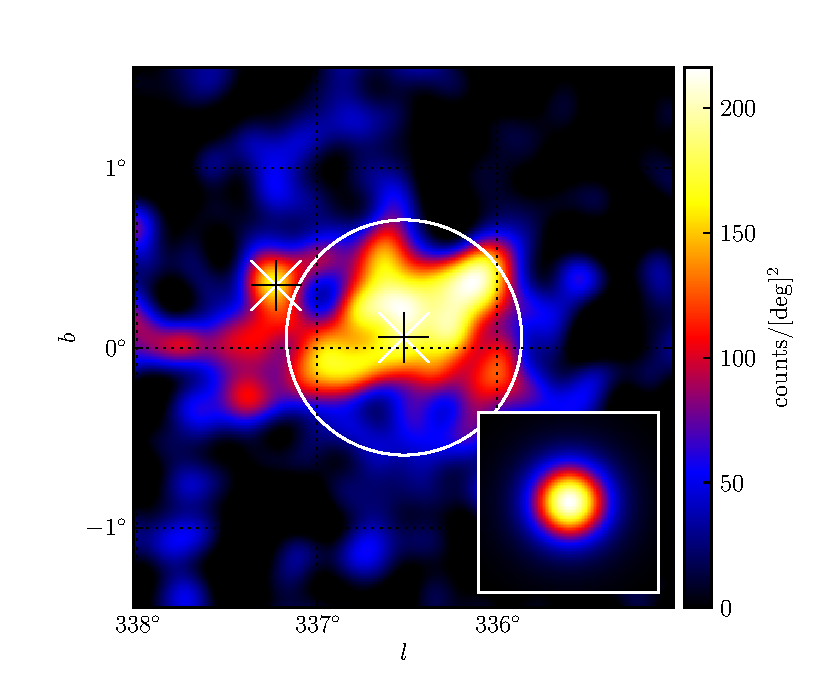
\includegraphics[type=pdf,ext=.pdf,read=.pdf]{source_plots/source_1FGL_J1632.9-4802c}
  \end{center}
  % this plot came from 
  % /u/gl/lande/work/fermi/extended_catalog/2FGL/plots_for_paper/source_plots/1FGL_J1632.9-4802c/v2/source_1FGL_J1632.9-4802c.pdf
  \caption{A Diffuse emission subtracted 10-100
  \gev counts map of the region around 2FGL\,J1632.4-4753c smoothed by
  a 0.1\deg Gaussian kernel.  This source is in a crowded region.
  The red star is the catalog position of this source.  The red
  cross and circle are the best fit position and extension 2FGL\,J1632.4-4753c 
  assuming a radially
  symmetric uniform surface brightness.
  The three
  green crosses inside the extension are 2FGL
  J1631.7-4720c, 2FGL\,J1630.2-4752, and 2FGL\,J1634.4-4743c.4-4820c
  which were removed because they are part
  of the extended source.  The blue stars and crosses are the catalog
  positions and the relocalized positions of (from left to right)
  2FGL\,J1635.4-4717c and 2FGL\,J1636.3-4740c.  The farther away green
  stars are other catalog sources which were removed because they are
  not significant above 10 \gev.  This extended source is spatially
  coincident with the extended H.E.S.S source HESS\,J1632-478.
  The light blue contours correspond to the \tev image observed by H.E.S.S.
  \citep{hess_plane_survey}.
  }\label{1FGL_J1632.9-4802c}
\end{figure}


\begin{figure}
  \begin{center}
    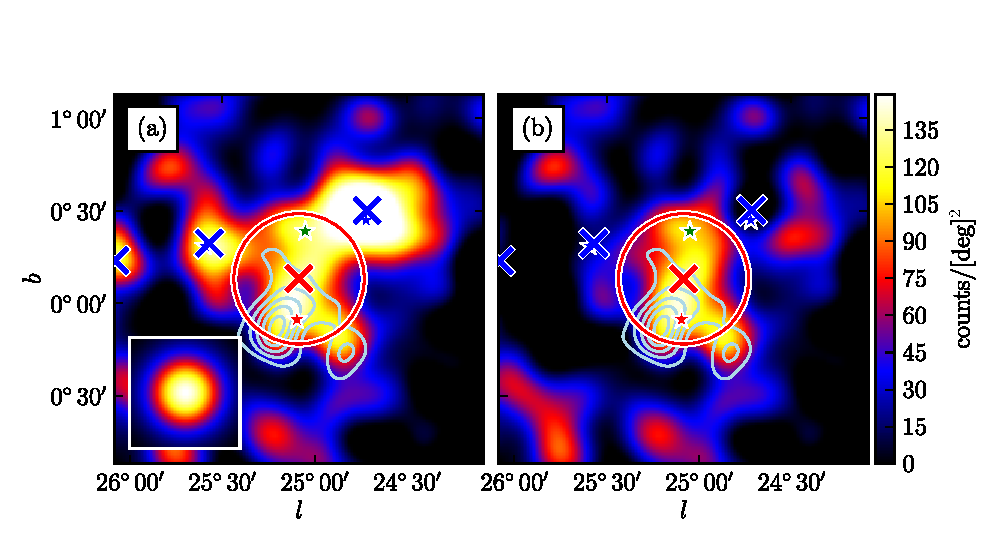
\includegraphics[type=pdf,ext=.pdf,read=.pdf]{source_plots/source_1FGL_J1837.5-0659c}
  \end{center}
  % this plot came from 
  % /u/gl/lande/work/fermi/extended_catalog/2FGL/plots_for_paper/source_plots/1FGL_J1837.5-0659c/v2/source_1FGL_J1837.5-0659c.pdf
  \caption{
  A Diffuse emission subtracted 10-100 \gev counts map of
  (a)
  the region around 2FGL\,J1837.3-0700c smoothed by a 0.1\deg Gaussian
  kernel and (b) also the emission from the background 
  sources subtracted.  The red
  star is the catalog position of this source. The red cross and circle
  are the best fit position and extension  of 2FGL\,J1837.3-0700c 
  assuming a radially
  symmetric uniform surface brightness. The blue stars and crosses are the
  catalog position and the relocalized position of (from left to right)
  2FGL\,J1839.3-0558c, 2FGL\,J1836.8-0623c, and 2FGL\,J1834.7-0705c.
  The green cross inside the extension is 2FGL\,J1835.5-0649 which
  was removed because it is part of the extended source.  The farther
  away green star is 2FGL J1839.0-0539 which was removed because
  it is not significant above 10 \gev.  This source is spatially
  coincident with the \tev source HESS\,J1837-069.  The light blue
  contours correspond to the \tev image observed by H.E.S.S.
  \citep{hess_plane_survey}.}\label{1FGL_J1837.5-0659c}
\end{figure}


\begin{figure}
  \begin{center}
    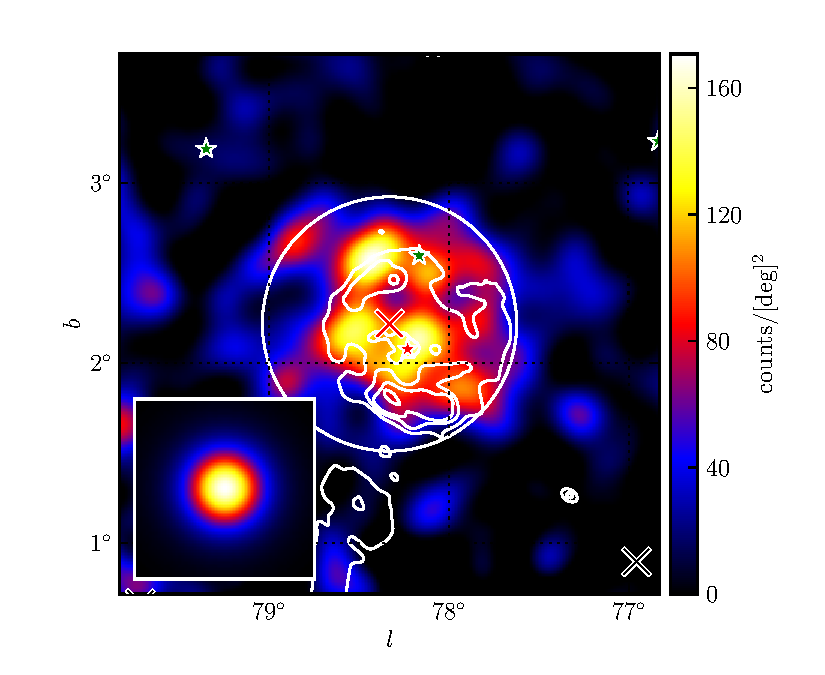
\includegraphics[type=pdf,ext=.pdf,read=.pdf]{source_plots/source_Gamma_Cygni}
  \end{center}
  % this plot came from 
  % /u/gl/lande/work/fermi/extended_catalog/2FGL/plots_for_paper/source_plots/Gamma_Cygni/v2/source_Gamma_Cygni.pdf
  \caption{A Diffuse subtracted 10-100 \gev counts map of the region
  around 2FGL\,J2021.5+4026 smoothed by a 0.1\deg Gaussian kernel. The
  red star is the catalog position of 2FGL J2021.5+4026.  The red cross
  and circle are the best fit position and extension 2FGL\,J2021.5+4026
  assuming a radially symmetric uniform surface brightness.  The green
  cross inside the extension is 2FGL\,J2019.1+4040 which was removed
  because it is part of the extended source.  The farther away green
  stars represent other catalog sources which were removed because
  they were not significant above 10 \gev.  The gray cross is the
  position a source not in the two year catalog which was added to the
  region. 2FGL\,J2021.5+4026 is spatially coincident with the $\gamma$
  Cygni SNR.  The light blue contours correspond to the 408MHz image of
  $\gamma$ Cygni observed by the Canadian Galactic Plane Survey.
  }\label{1FGL_J2020.0+4049}
\end{figure}

\clearpage
\begin{figure}
  \begin{center}
    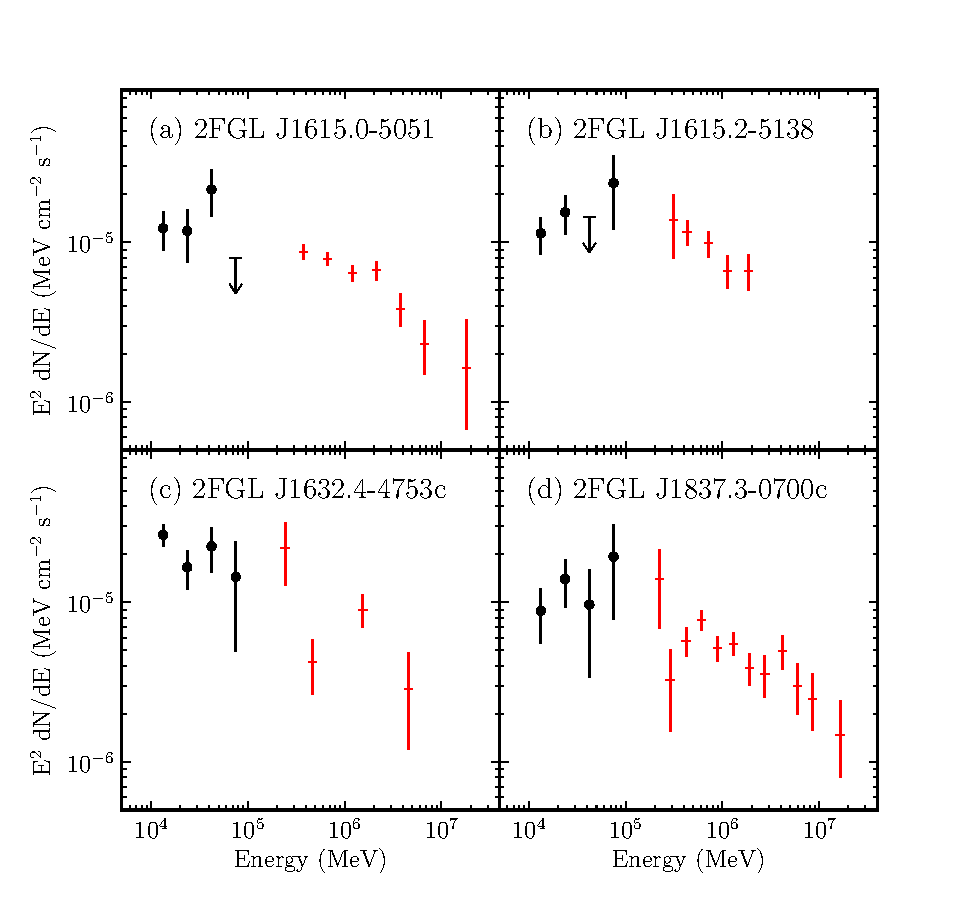
\includegraphics{summary_plots/hess_seds.pdf}
    % this plot came from /u/gl/lande/work/fermi/extended_catalog/2FGL/seds/v3/plot_seds/plot_seds.py
    \end{center}
    \caption{
    The spectral energy distribution of four the extended sources
    associated with extended \tev sources.  The black points with circular
    markers are the LAT data points. The red points with dashed markers
    are H.E.S.S points of associated sources.  Plot (a) shows the \gev
    SED of 2FGL\,J1615.0-5051 together with the \tev SED of HESS\,J1616-508.
    Plot (b) shows 2FGL\,J1615.2-5138 and HESS\,J1614-518 Plot (c)
    shows 2FGL\,J1632.4-4753c and HESS\,J1632-478. Plot (d) shows
    2FGL\,J1837.3-0700c and HESS\,J1837-069. The H.E.S.S. data points
    are from \citep{hess_plane_survey} The LAT upper limits are at the
    95\% confidence level.  Both LAT and H.E.S.S. spectral errors are
    systematic only.}
    \label{hess_seds}
  \end{figure}

\clearpage
{\rotate
\begin{figure}
  \begin{center}
    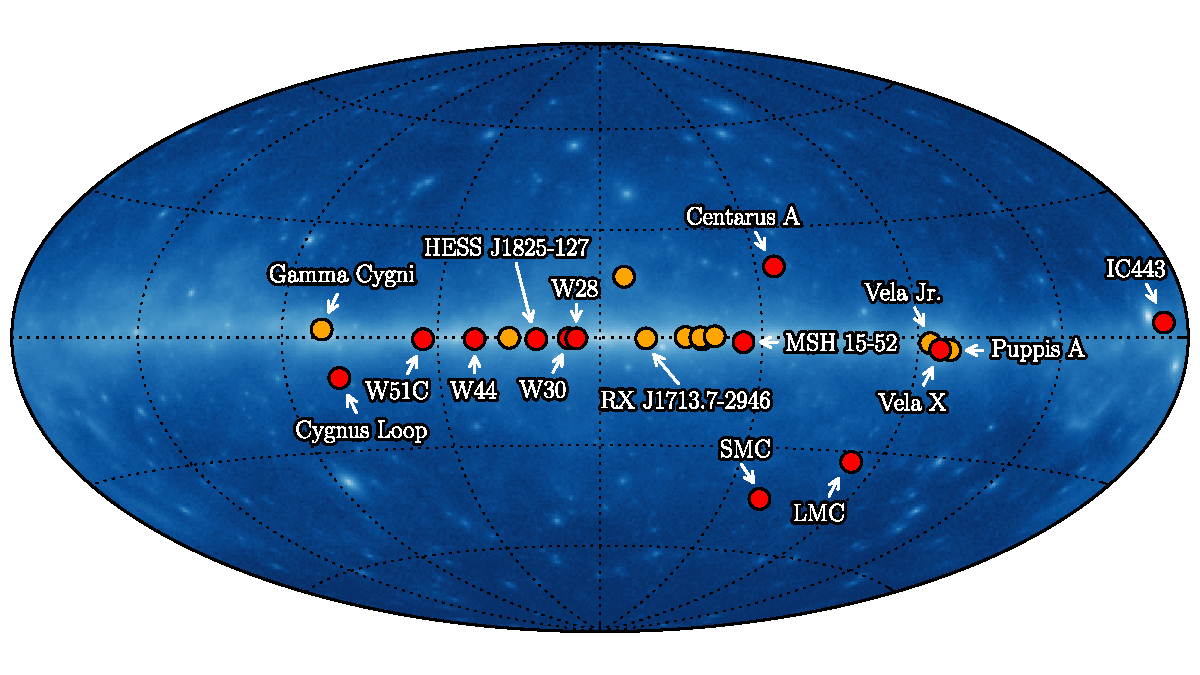
\includegraphics{summary_plots/allsky_extended_sources.pdf}
    % this plot came from /u/gl/lande/work/fermi/extended_catalog/2FGL/plots_for_paper/allsky/v1/run.py
    \end{center}
    \caption{A plot of all \gev extended sources detected by the LAT
    with two years of data.  The twelve extended sources included in
    2FGL are the red markers and the nine additional
    extended sources analyzed in this paper are the orange markers. 
    }\label{allsky_extended_sources}
  \end{figure}
  }


\clearpage
\begin{figure}
  \begin{center}
    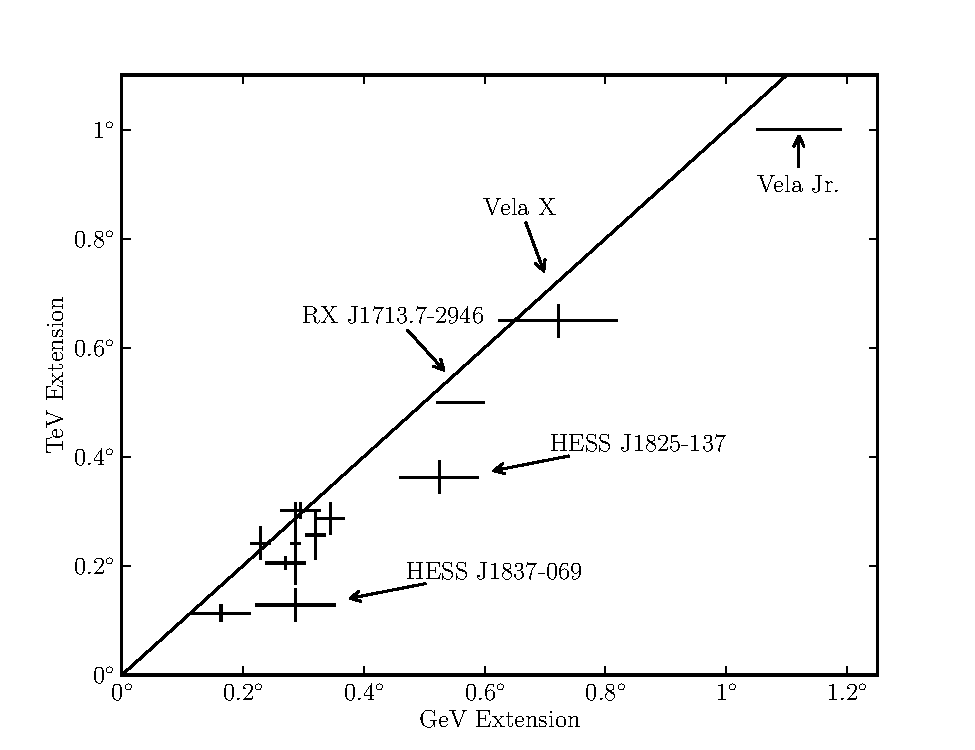
\includegraphics{summary_plots/gev_vs_tev_plot.pdf}
    % this plot came from /u/gl/lande/work/fermi/extended_catalog/2FGL/plots_for_paper/compare_tev_gev_sizes/v1/run.py
    \end{center}
    \caption{
    A comparison of the \gev and \tev sizes of LAT extended
    sources detected by \tev instruments.  The \tev extensions
    of W30, 2FGL\,J1837.3-0700c, 2FGL\,J1632.4-4753c,
    2FGL\,J1615.0-5051, and 2FGL\,J1615.2-5138 \citep{hess_plane_survey}.
    The \tev extensions of MSH 15-52, HESS\,J1825-137, Vela X,
    Vela Jr., RX J1713.7-3946 and W28 are from 
    \citep{msh_15_52_hess,hess_j1825_hess,vela_x_hess,vela_jr_hess,rx_j1713_hess,w28_hess}.
    The \tev extension of IC443 is from \citep{ic443_veritas}
    and W51c is from \citep{w51c_with_magic_at_fermi_symposium}.
    The LAT extension of Vela X is from \citep{velax}.  Except for RX
    J1713.7-3946 Vela Jr., the \tev sources were fit assuming a Gaussian
    surface brightness so the plotted \gev and \tev extensions were first
    converted to \rsixeight (see section~\ref{compare_source_size}).
    Because of their large size, the shape of RX J1713.7-3946 and Vela Jr.
    were not directly fit in \tev. Here, we take their
    sizes to be the same as the LAT size and 
    do not converted it to \rsixeight. The LAT extension errors are
    the statistical and systematic errors added in quadrature. The \tev size of MSH 15-52, HESS\,J1614-518,
    HESS\,J1632-478, and HESS\,J1837-069 have only been reported with
    an elliptical Gaussian fit and so the plotted size is the average
    of semi-major and semi-minor axis.
    }\label{gev_vs_tev_plot}
  \end{figure}

\clearpage
\begin{figure}
  \begin{center}
    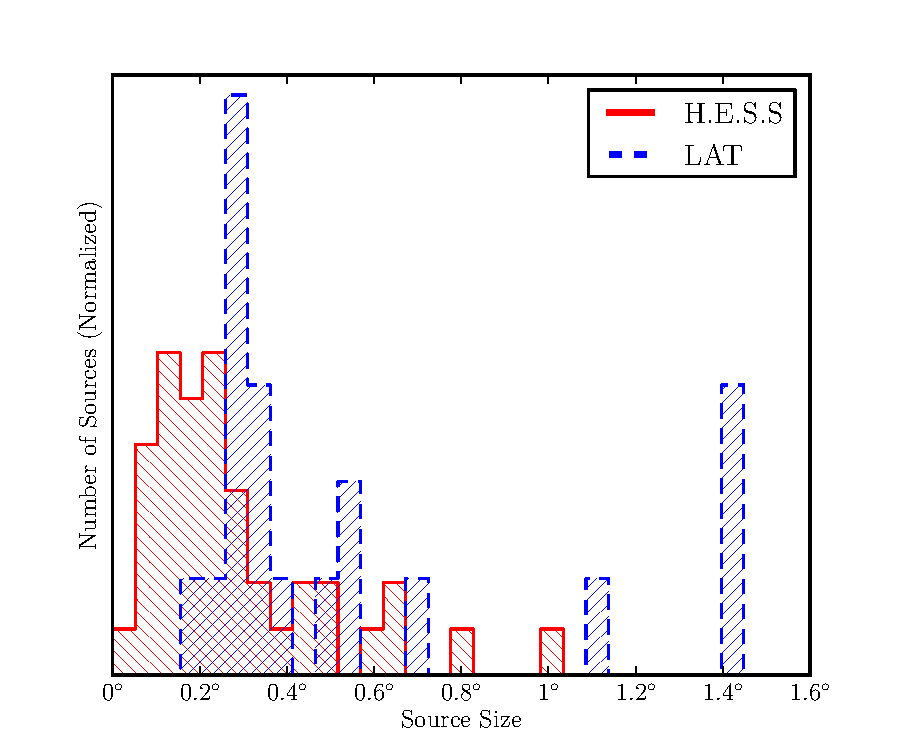
\includegraphics{summary_plots/gev_vs_tev_histogram.pdf}
    % this plot came from /u/gl/lande/work/fermi/extended_catalog/2FGL/plots_for_paper/extension_histogram/v4/extension_histogram.py
    \end{center}
    \caption{
    A comparison of the size of detected LAT and H.E.S.S sources.
    The extension of the 22 extended LAT sources comes from
    table~\ref{known_extended_sources}, table~\ref{new_ext_srcs_table},
    and the LAT extension of Vela X is taken from \citep{velax}. The
    The \tev extension of
    the 42 extended H.E.S.S. sources comes from the H.E.S.S. Source
    Catalog \citep{hesscat}.
    Except for RX J1713.7-3946 and Vela Jr.,
    the H.E.S.S. sources were fit with a Gaussian surface
    brightness model and
    so the LAT and H.E.S.S. sizes are first converted to \rsixeight.
    (see section~\ref{compare_source_size}). Because the spatial
    morphology of RX J1713.7-3946 and Vela Jr. is poorly matched by a
    Gaussian surface brightness model, the \gev and
    \tev extensions are assuming a uniform surface brightness.
    }\label{gev_vs_tev_histogram}
  \end{figure}

\clearpage
\begin{figure}
  \begin{center}
    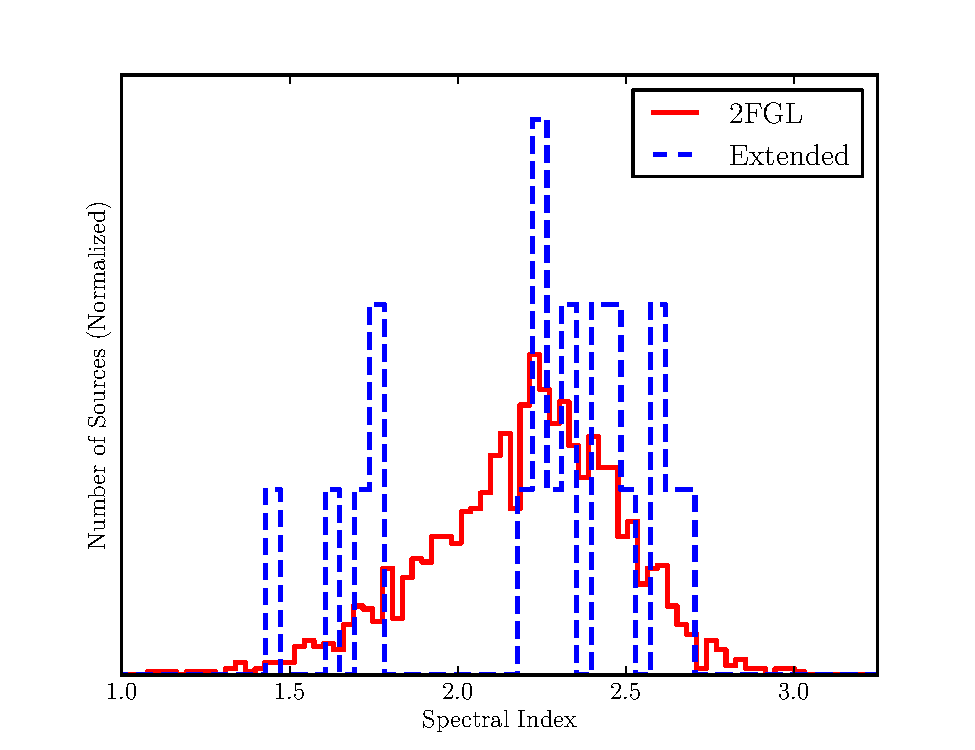
\includegraphics{summary_plots/compare_index_2FGL.pdf}
    % plot taken from /u/gl/lande/work/fermi/extended_catalog/2FGL/plots_for_paper/compare_index_2fgl/v3/run.py
    \end{center}
    \caption{
    The distribution of spectral indices of all 1873 2FGL sources in
    red and all spatially extended sources in blue. The
    spectral indices of LAT extended sources are taken from
    table~\ref{known_extended_sources} table~\ref{new_ext_srcs_table}.
    The index of Centarus A is taken to be 2.58 from 
    \cite{second_cat} and the index of Vela X is taken to be 2.41
    from \cite{velax}. }\label{compare_index_2FGL}
  \end{figure}



\end{document}
